%%%%%%%%%%%%%%%%%%%%%%%%%%%%%%%%%%%%%%%%%%%%%%%%%%%%%%%%%%%%%%%%%%%%%%%%%%%%%%%%%%%%%%%%%
%
%
%       SECTION: NOISE DESCRIPTION
%
%
%%%%%%%%%%%%%%%%%%%%%%%%%%%%%%%%%%%%%%%%%%%%%%%%%%%%%%%%%%%%%%%%%%%%%%%%%%%%%%%%%%%%%%%%%


%----------------------------------------------------------------------
%
%    
%
%---------------------------------------------------------------------
\subsection{Noise power spectrum}


%----------------------------------------------------------------------
%
%     KID-KID correlation matrix
%
%     copied from v0/dark_tests.tex, Juan
%
%---------------------------------------------------------------------

\subsection{Detector-Detector correlation matrix}

For this work we have used several decorrelation methods trying to identify possible multiple components in the noise. Notice that in the following the atmospheric signal will be considered simply as correlated sky noise. The main decorrelation methods used are:

\begin{enumerate}
\item[CM] {\bf Common mode decorrelation}. We search for a common mode template using all detectors of the same array. To avoid bias from bad detectors we consider the median common mode.

\item[PCA] {\bf Principal Component Analysis}. For each NIKA2 array independently we decompose the covariance matrix in principal components. From those we derive up to 10 independent templates corresponding to the largest eigenvalue values.

\item[BC] {\bf Best correlated pixels}. For each detector in a given array we identify those detectors which are more correlated to it (a minimum of 14). Using those detectors we compute a common mode as in method CM. 

\item[ALL] {\bf All detectors}. For earch detector of a given array we use all other detectors of the same array as templates and perform a linear fit.

\end{enumerate}

In Figure~\ref{corrs72} we show the noise correlation matrices for the N2R7 faint source scan 20161213s72. As expected the raw data noise correlation is dominated by atmospheric noise and we observe full correlation between detectors. After decorrelation the results are very similar to those found for N2R7 dark scan 20161211s299. There is residual significant correlation and anti-correlation after CM decorrelation. PCA decorrelation leads to a more diagonal correlation matrices. For the BC decorrelation the results are worse (more residual correlation and anti-correlation) and close to those of the CM decorrelation. As before there are good indications of multiple electronic-detector noise components. It is interesting to note that the detector-electronic noise correlation patterns seems to be the same for dark tests and for sky data. 


\begin{figure}[ht] % Inline image example
\begin{center}
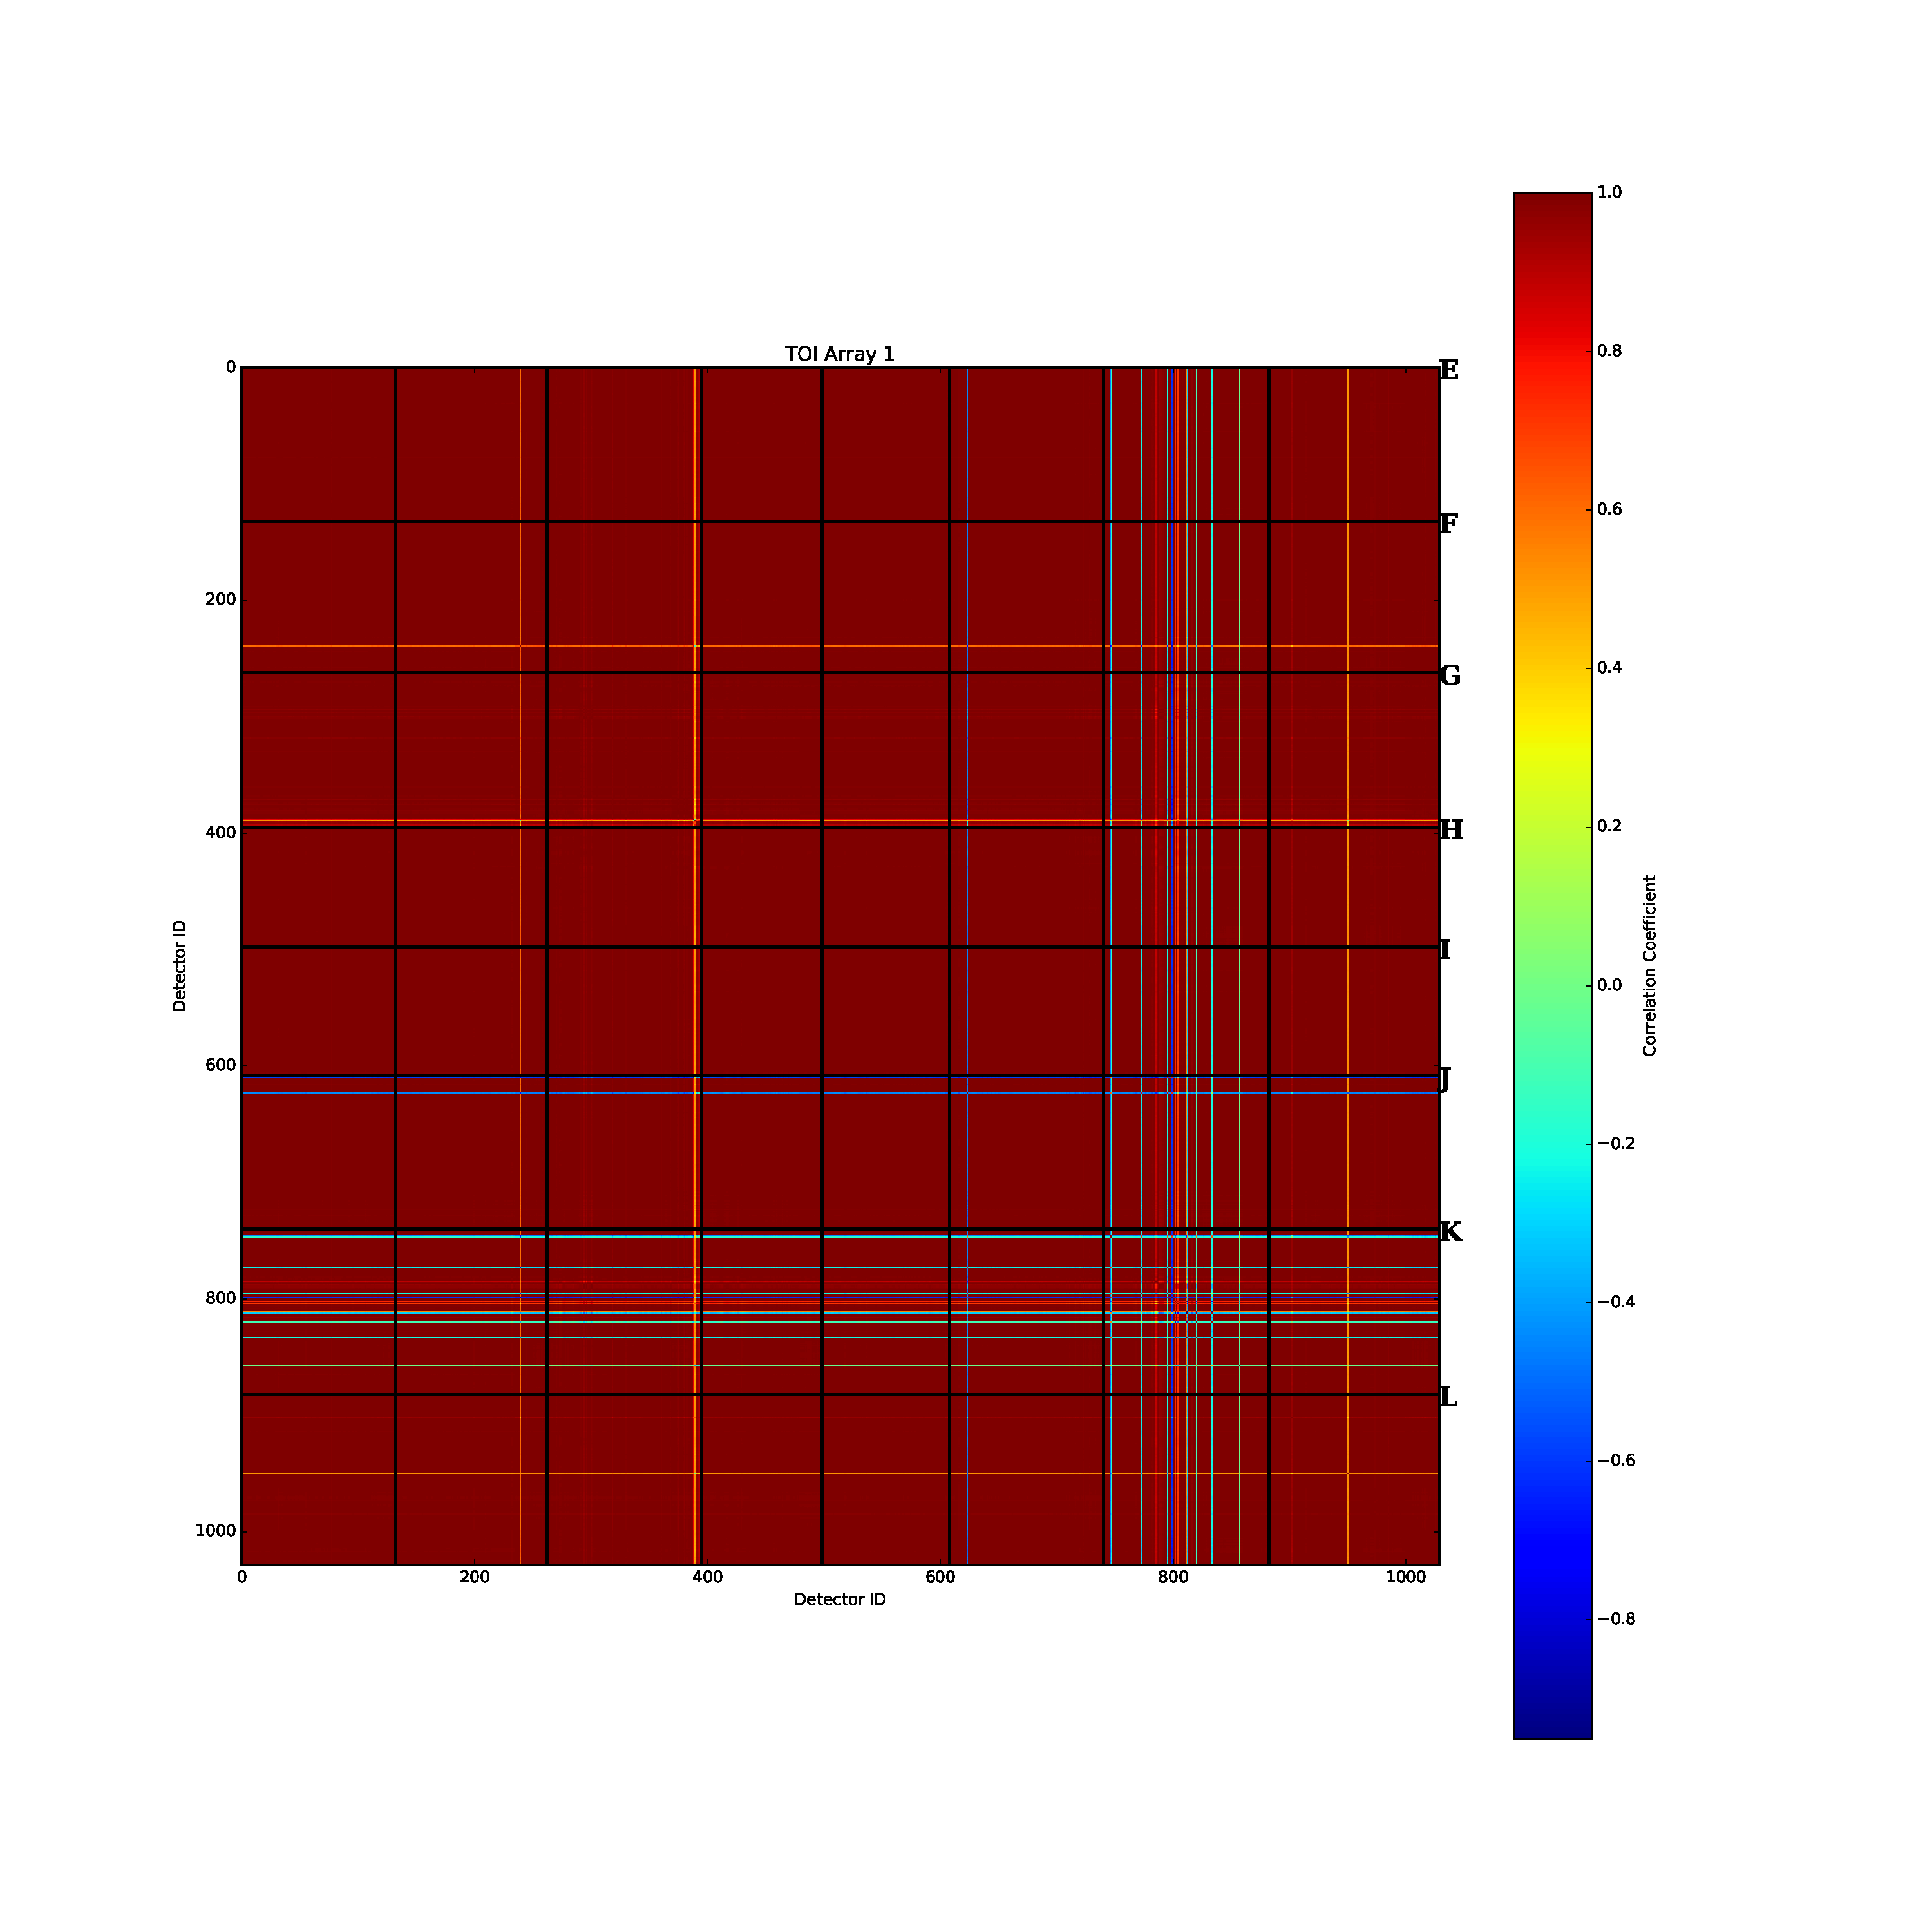
\includegraphics[width=0.3\textwidth]{Figures/DarkTests/corrmat_TOI_array_1_20161213s72.pdf}
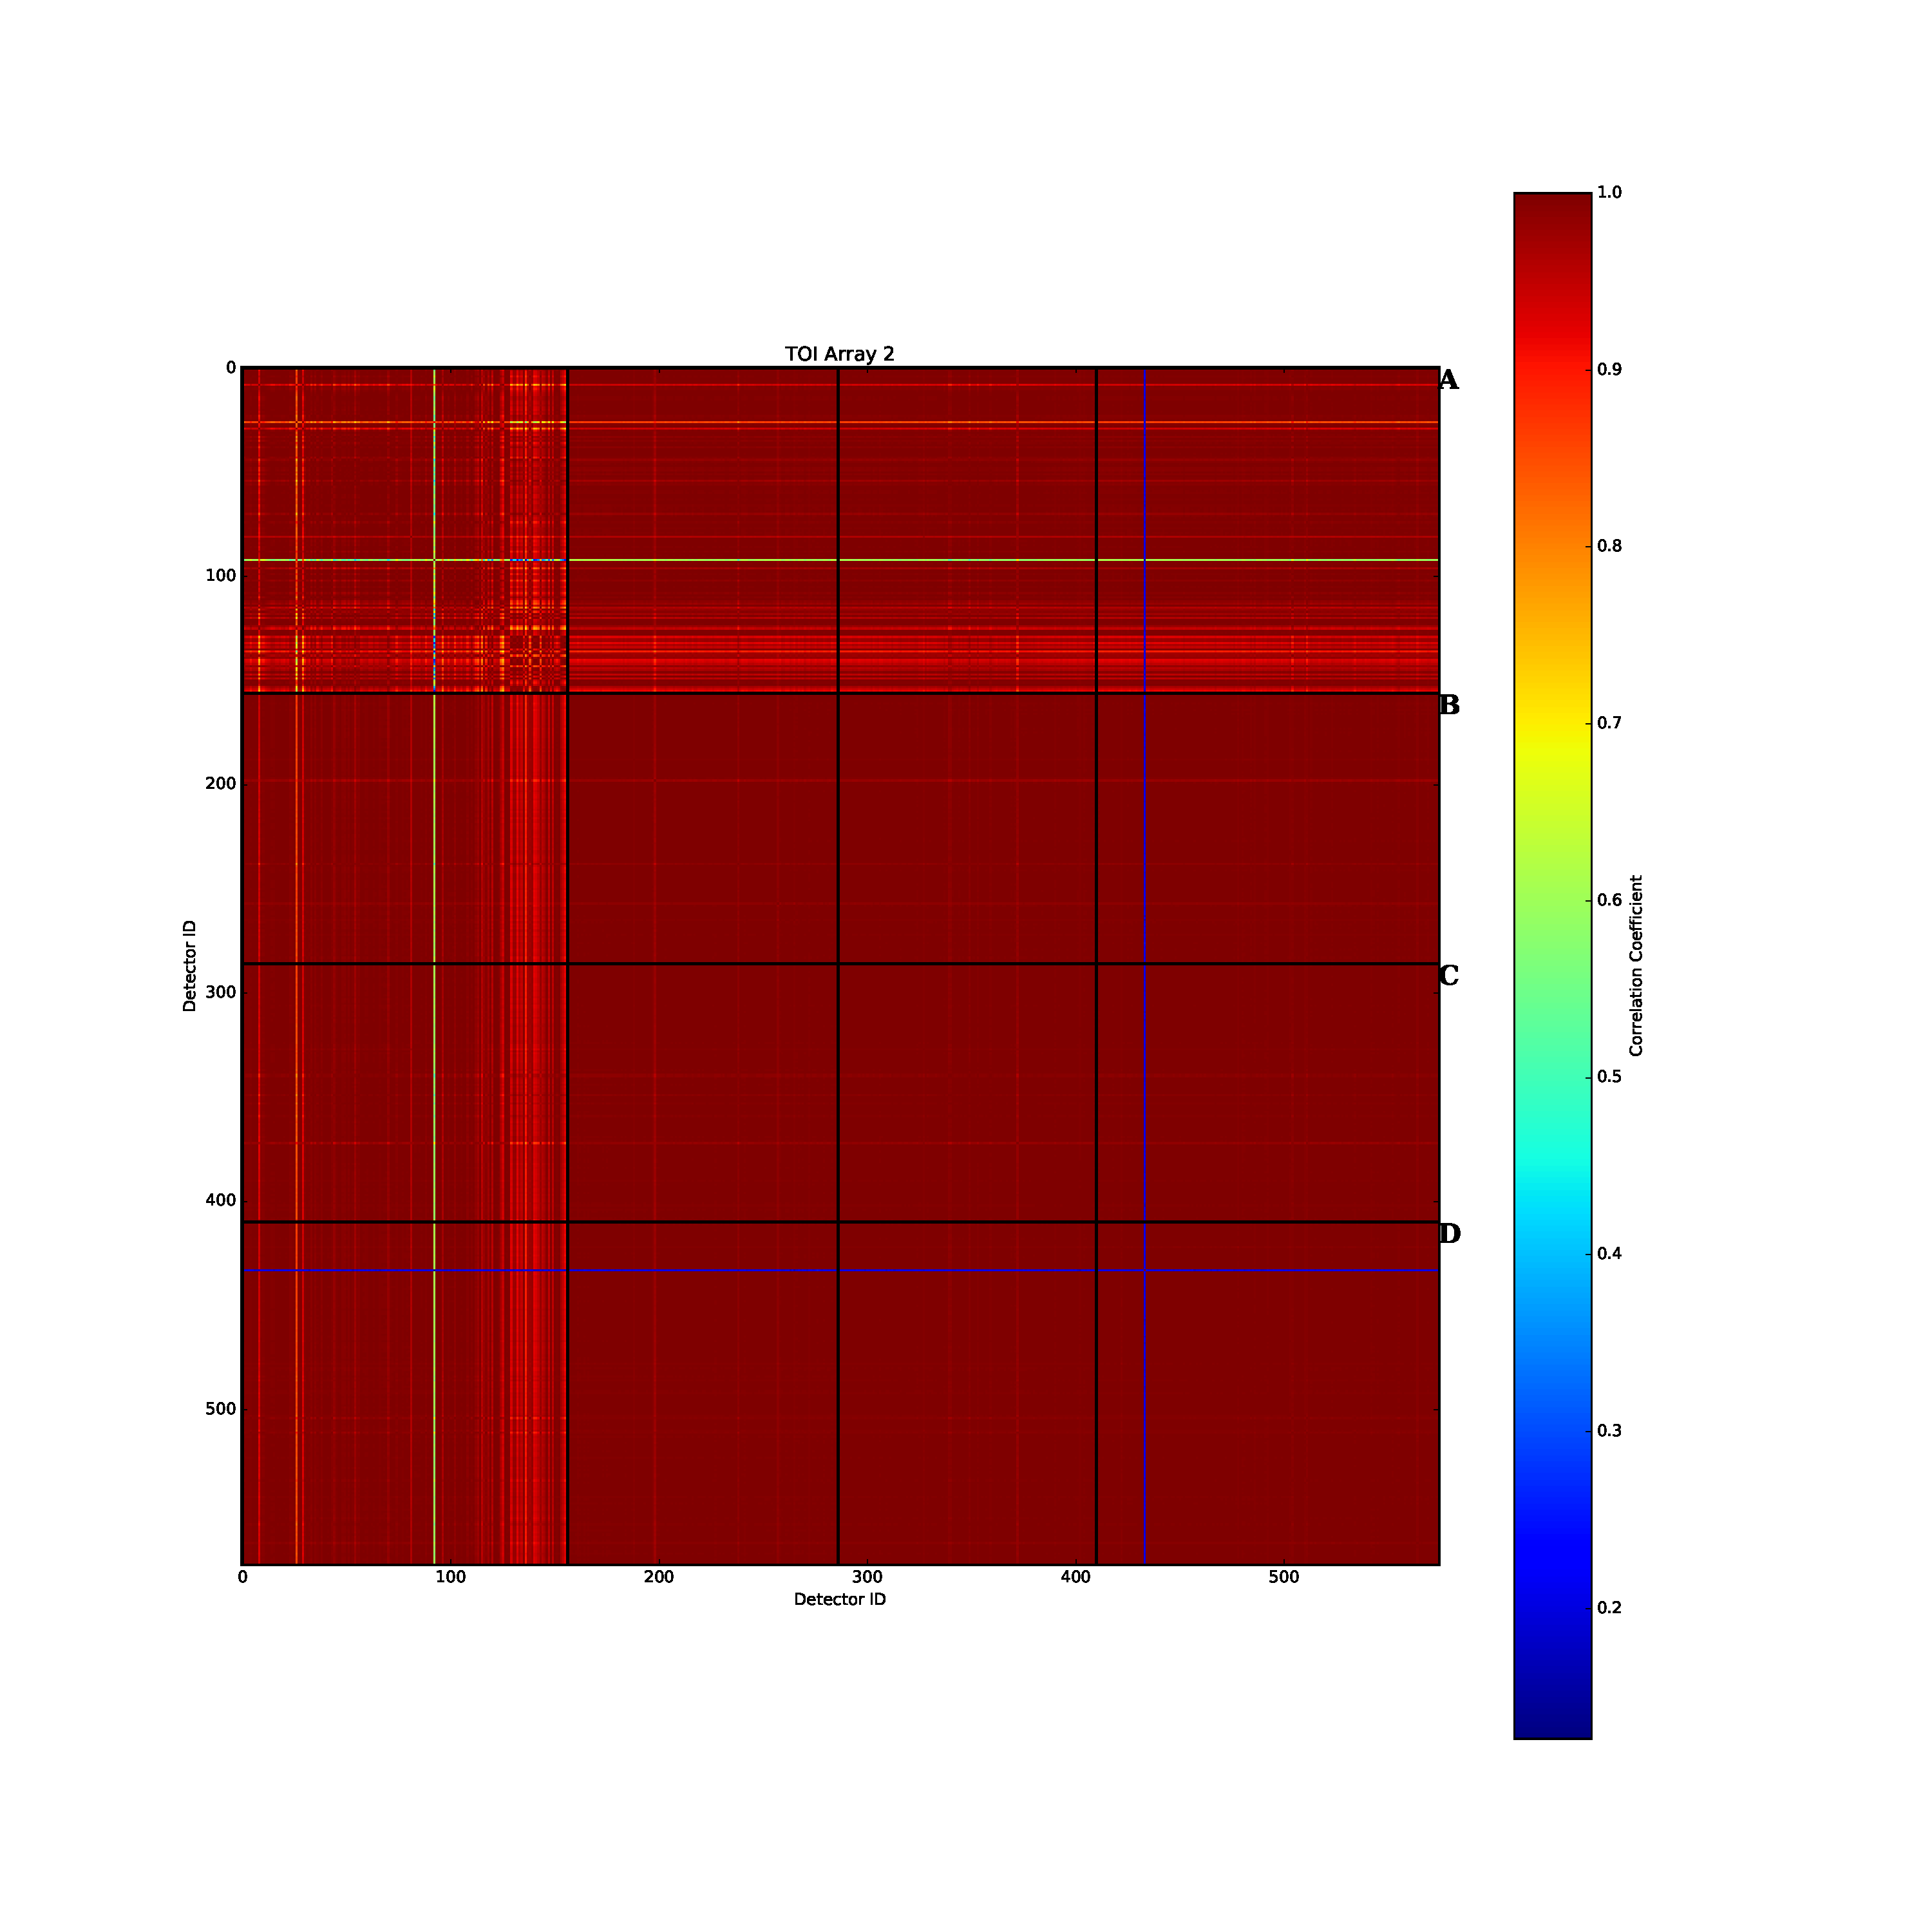
\includegraphics[width=0.3\textwidth]{Figures/DarkTests/corrmat_TOI_array_2_20161213s72.pdf}
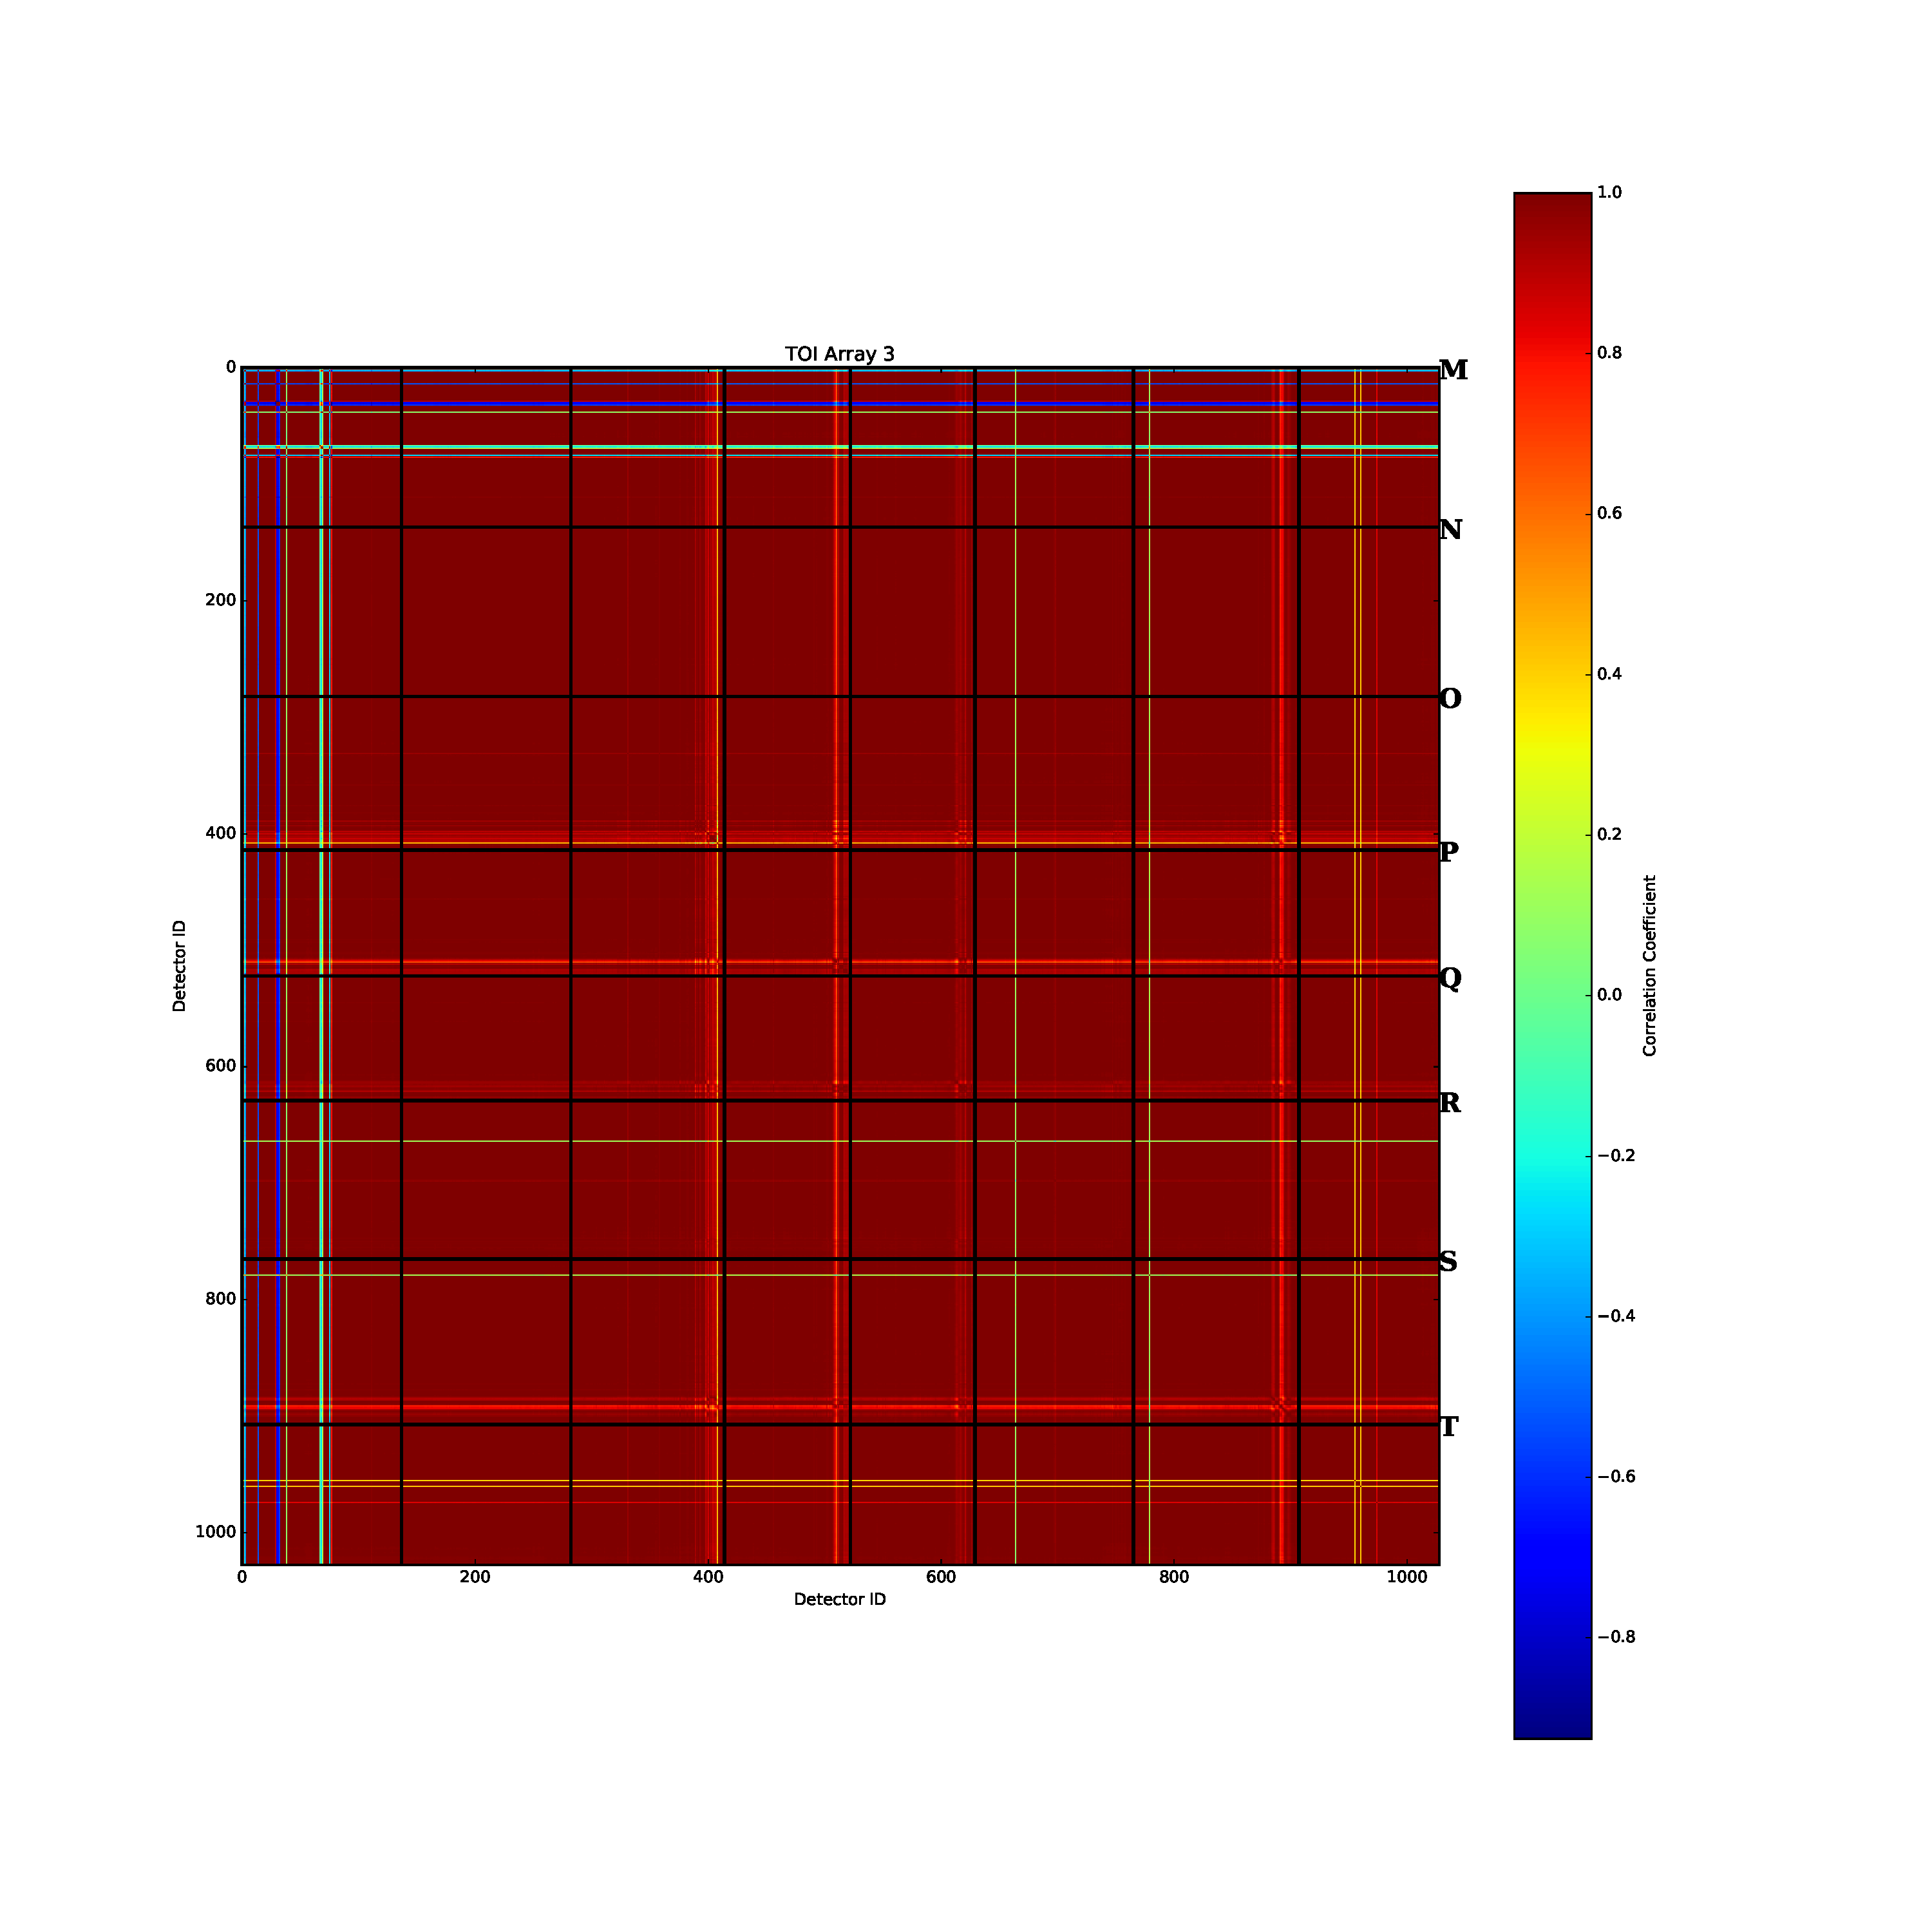
\includegraphics[width=0.3\textwidth]{Figures/DarkTests/corrmat_TOI_array_3_20161213s72.pdf}
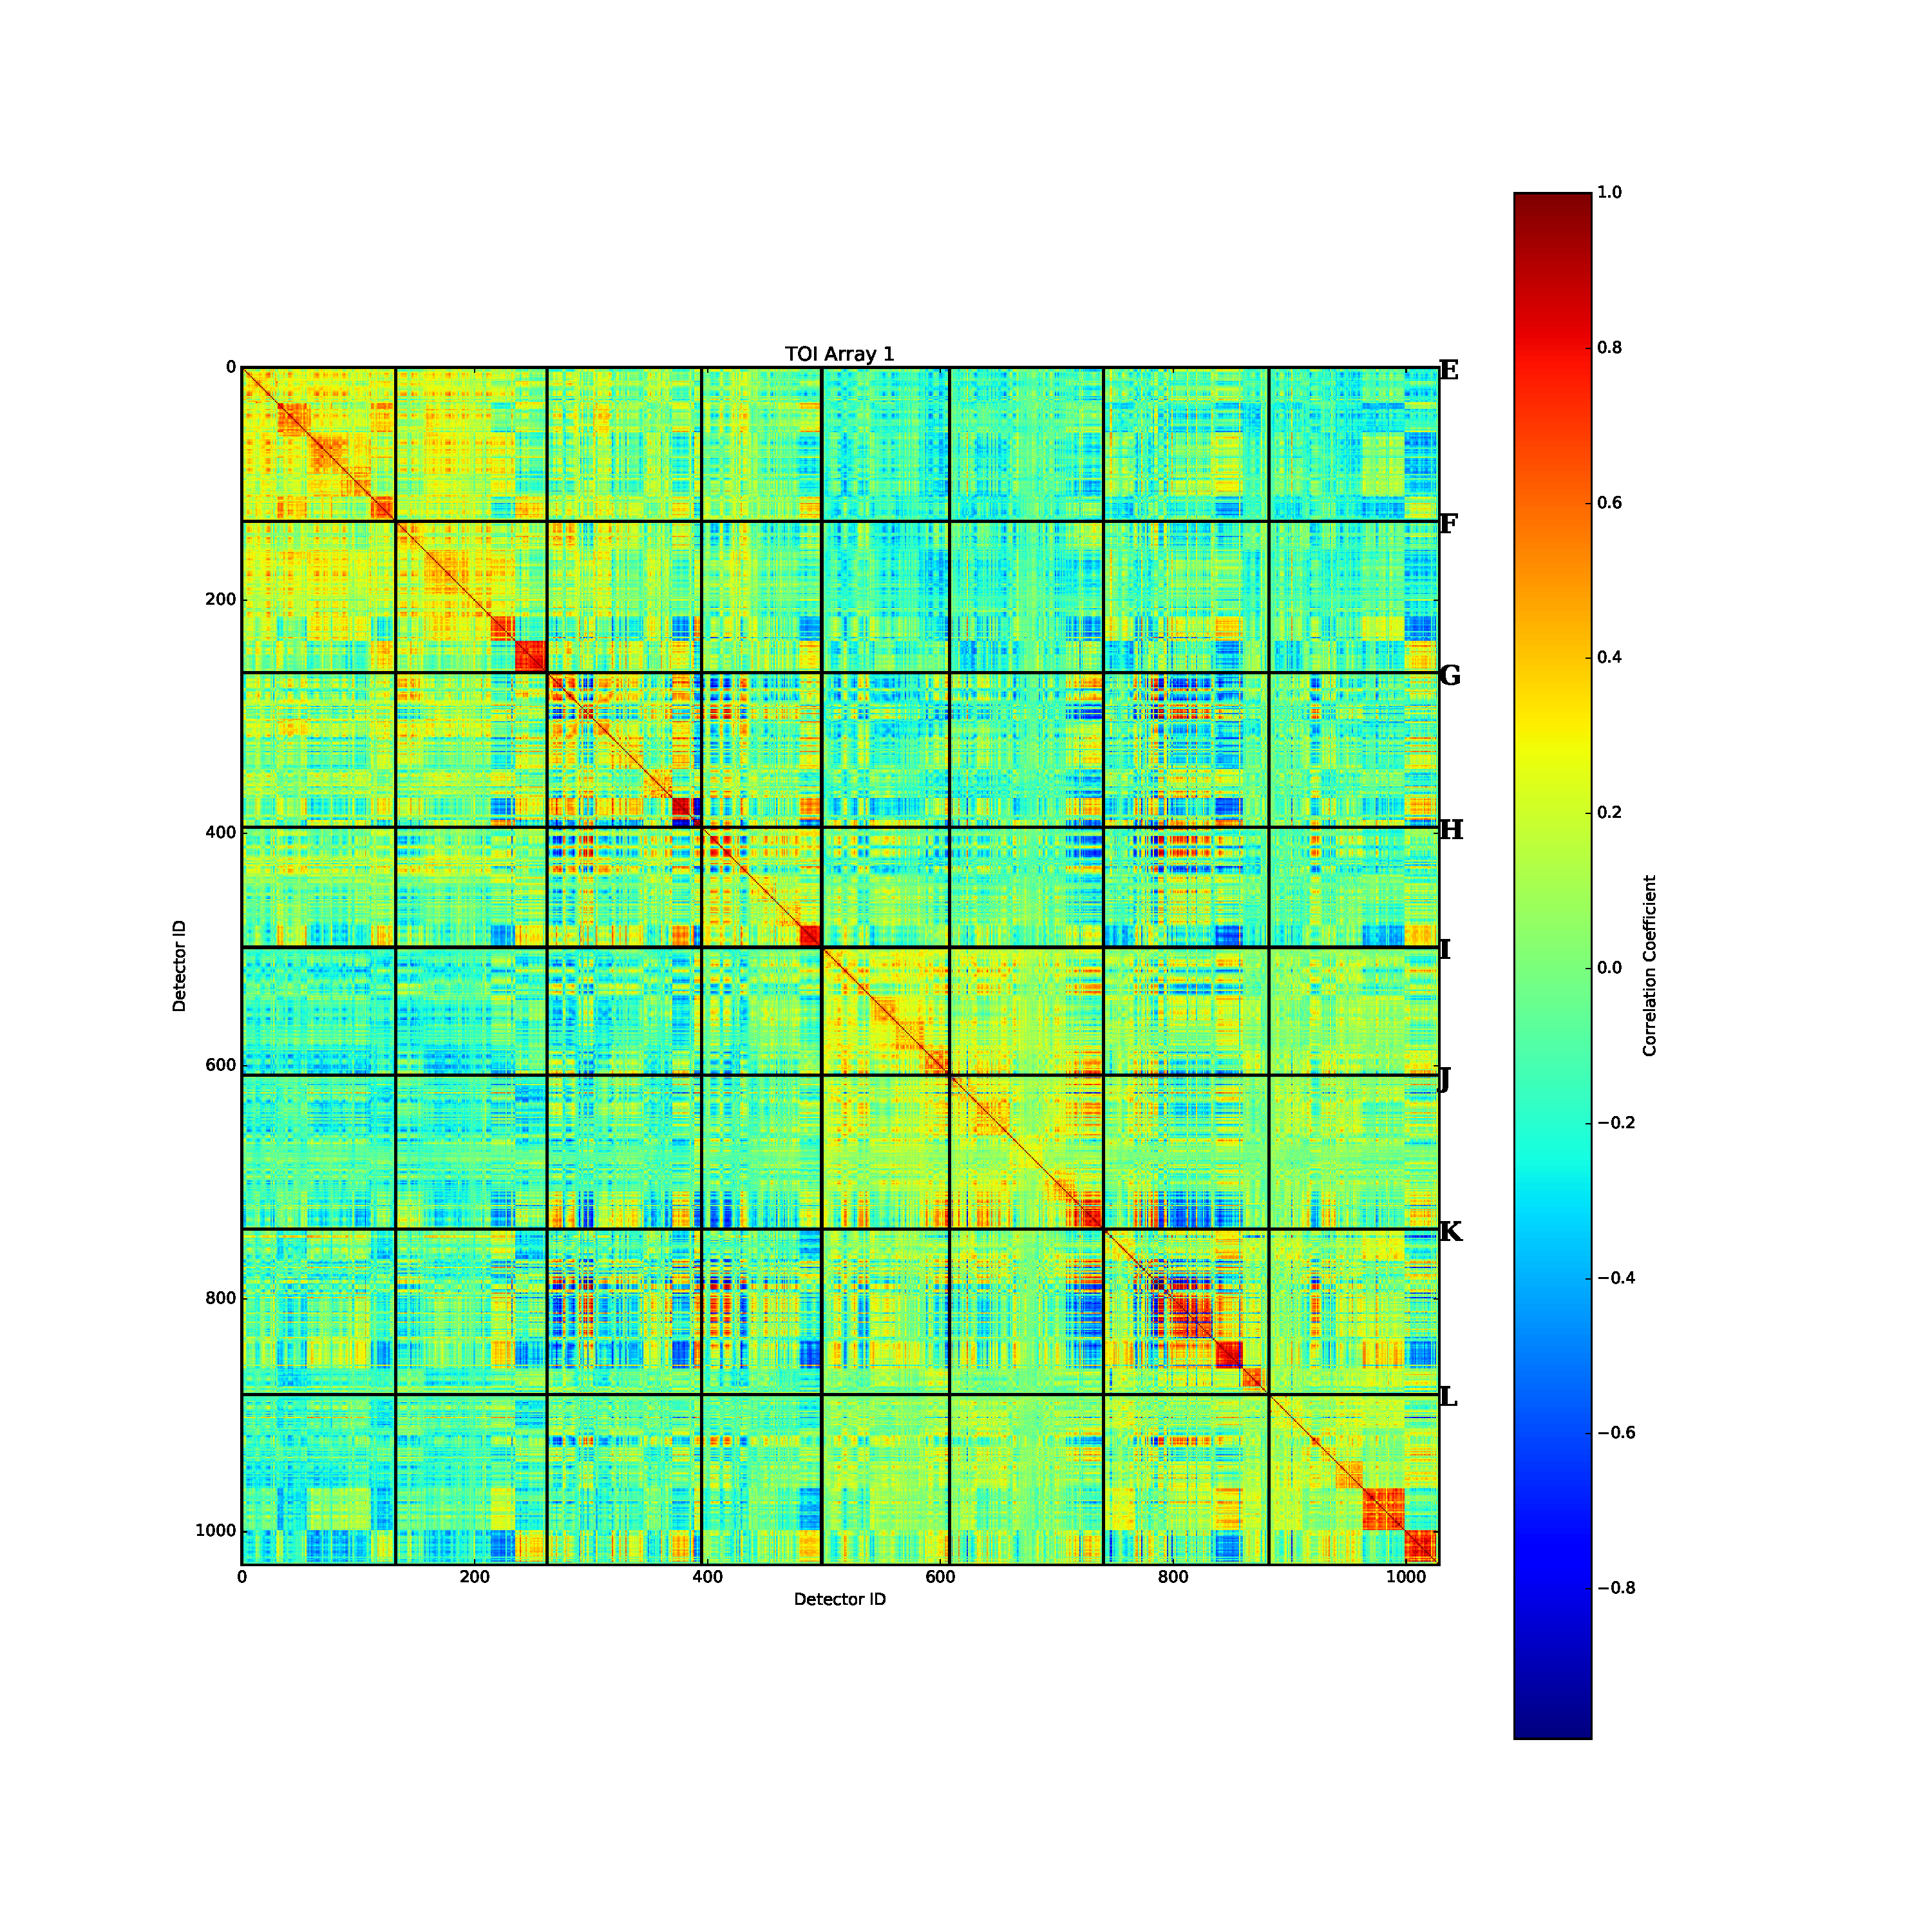
\includegraphics[width=0.3\textwidth]{Figures/DarkTests/corrmat_TOI_CM_array_1_20161213s72.pdf}
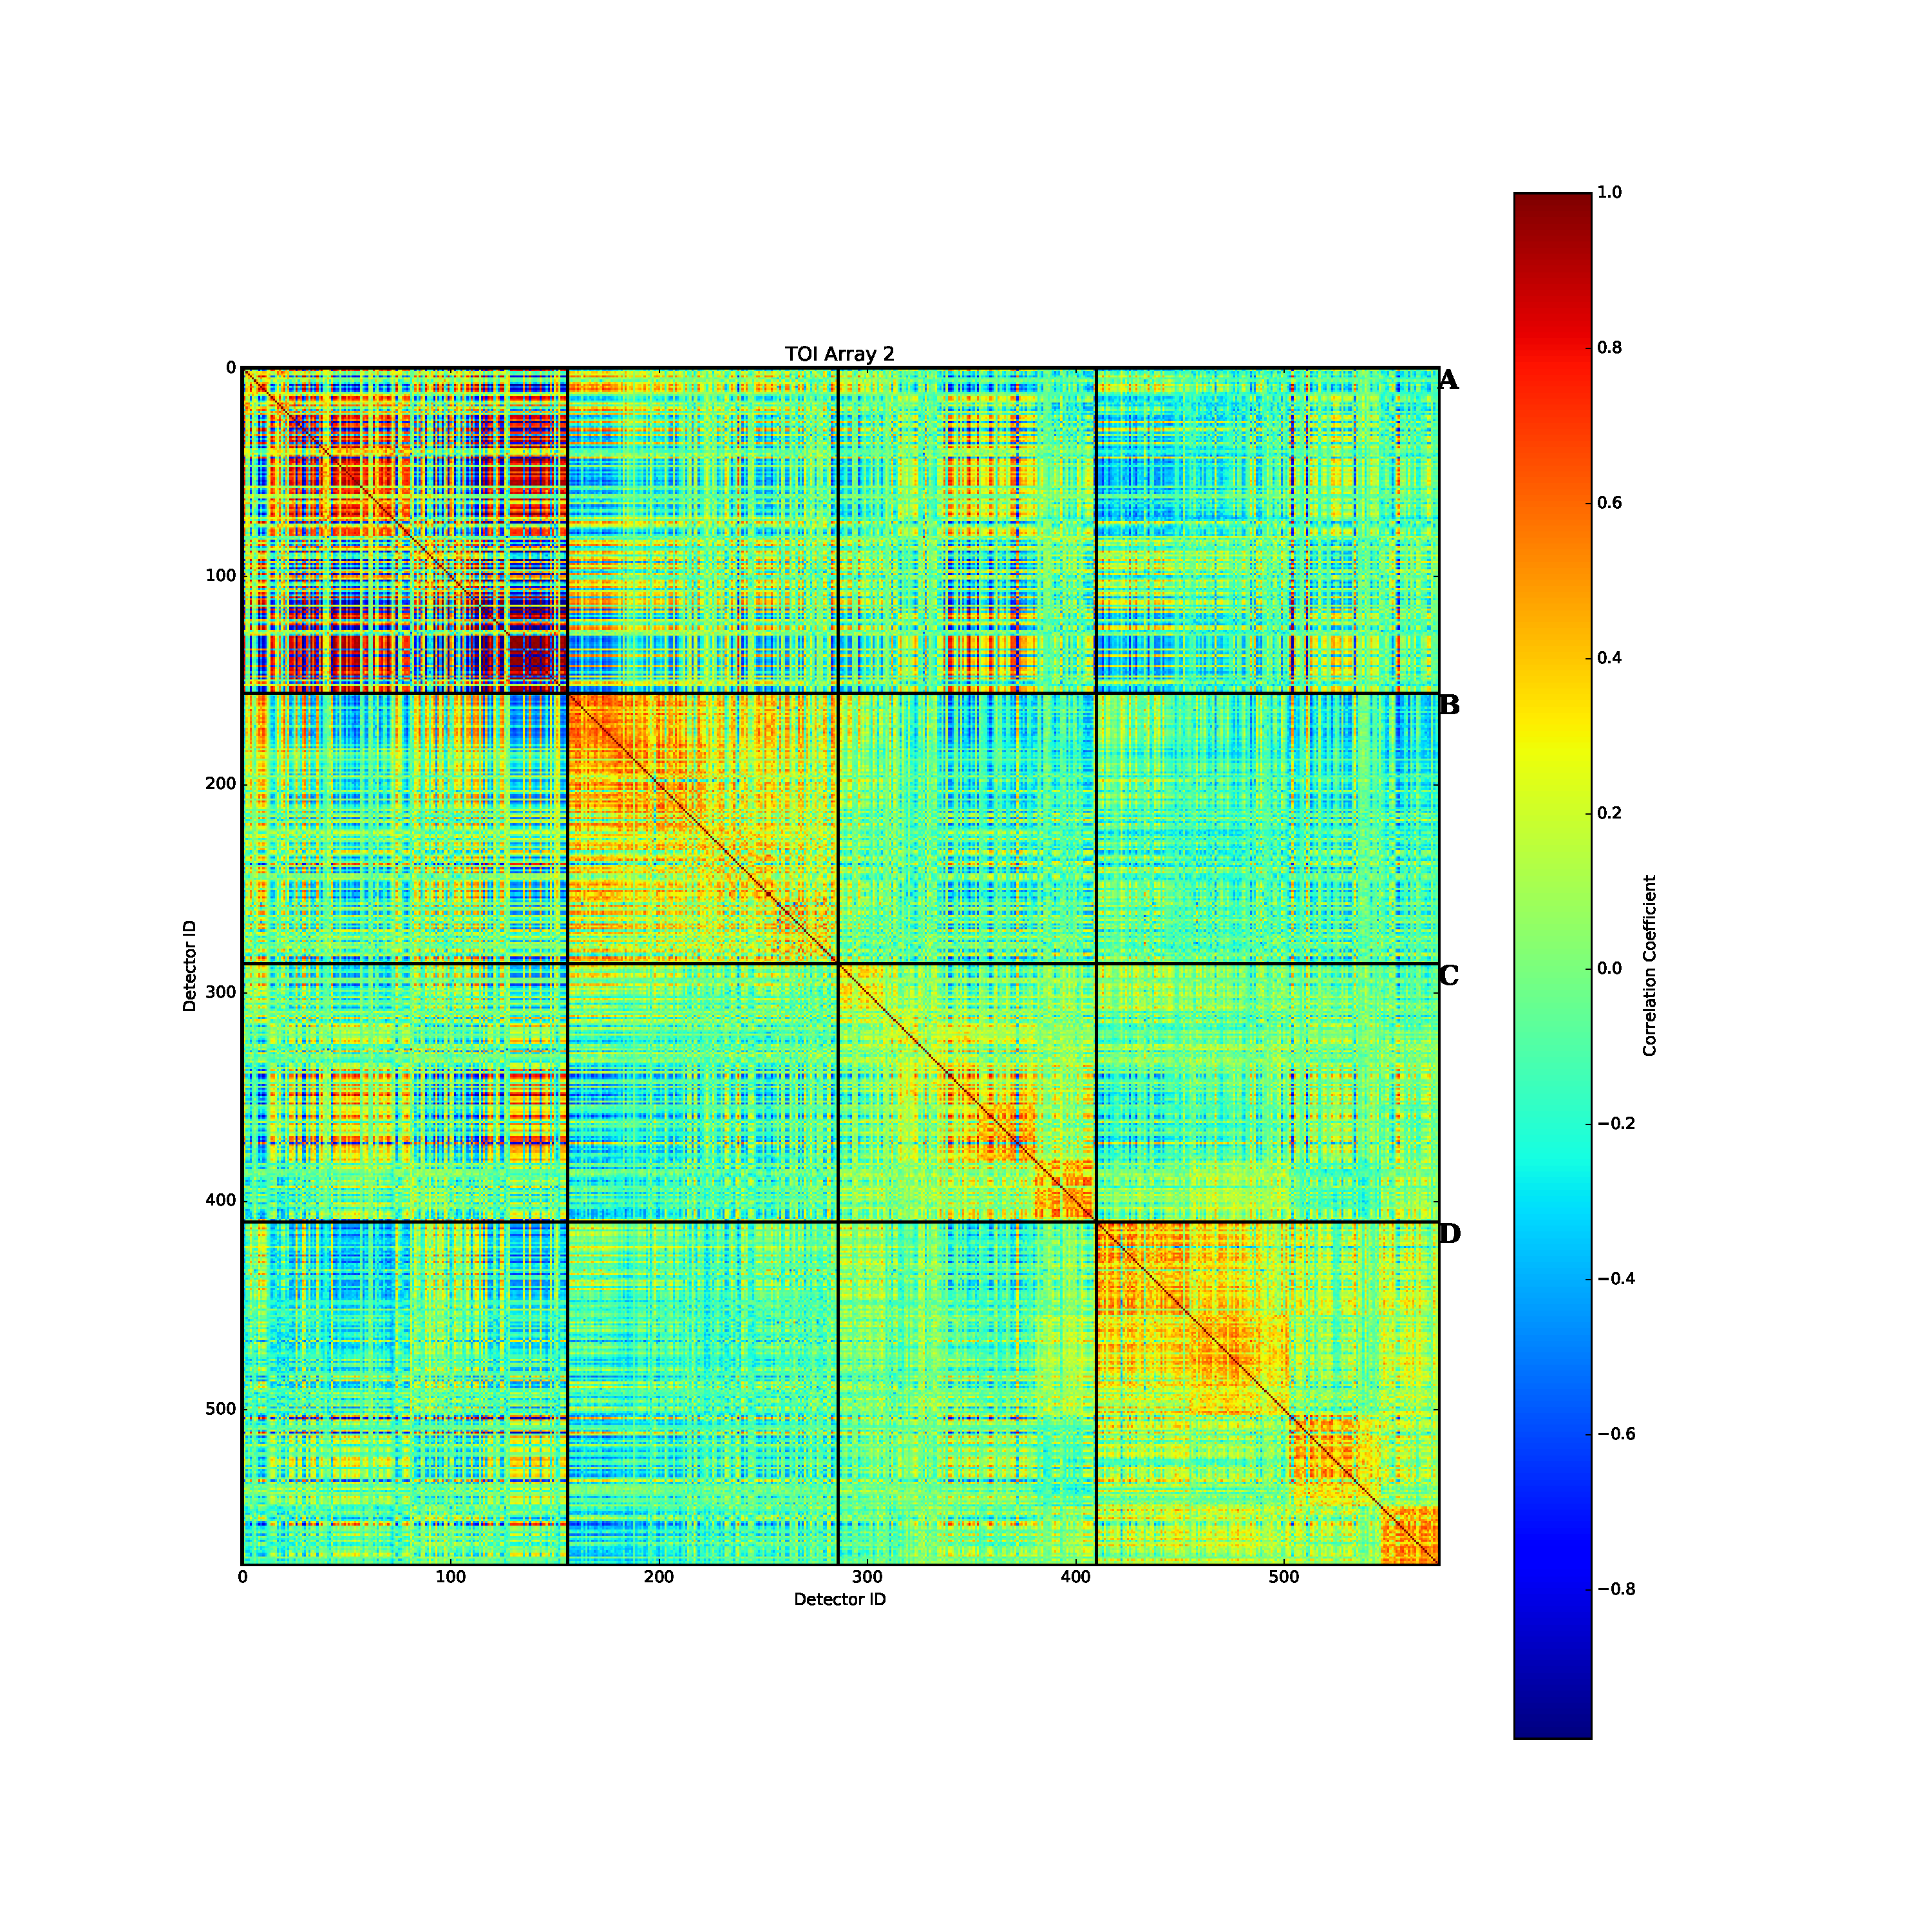
\includegraphics[width=0.3\textwidth]{Figures/DarkTests/corrmat_TOI_CM_array_2_20161213s72.pdf}
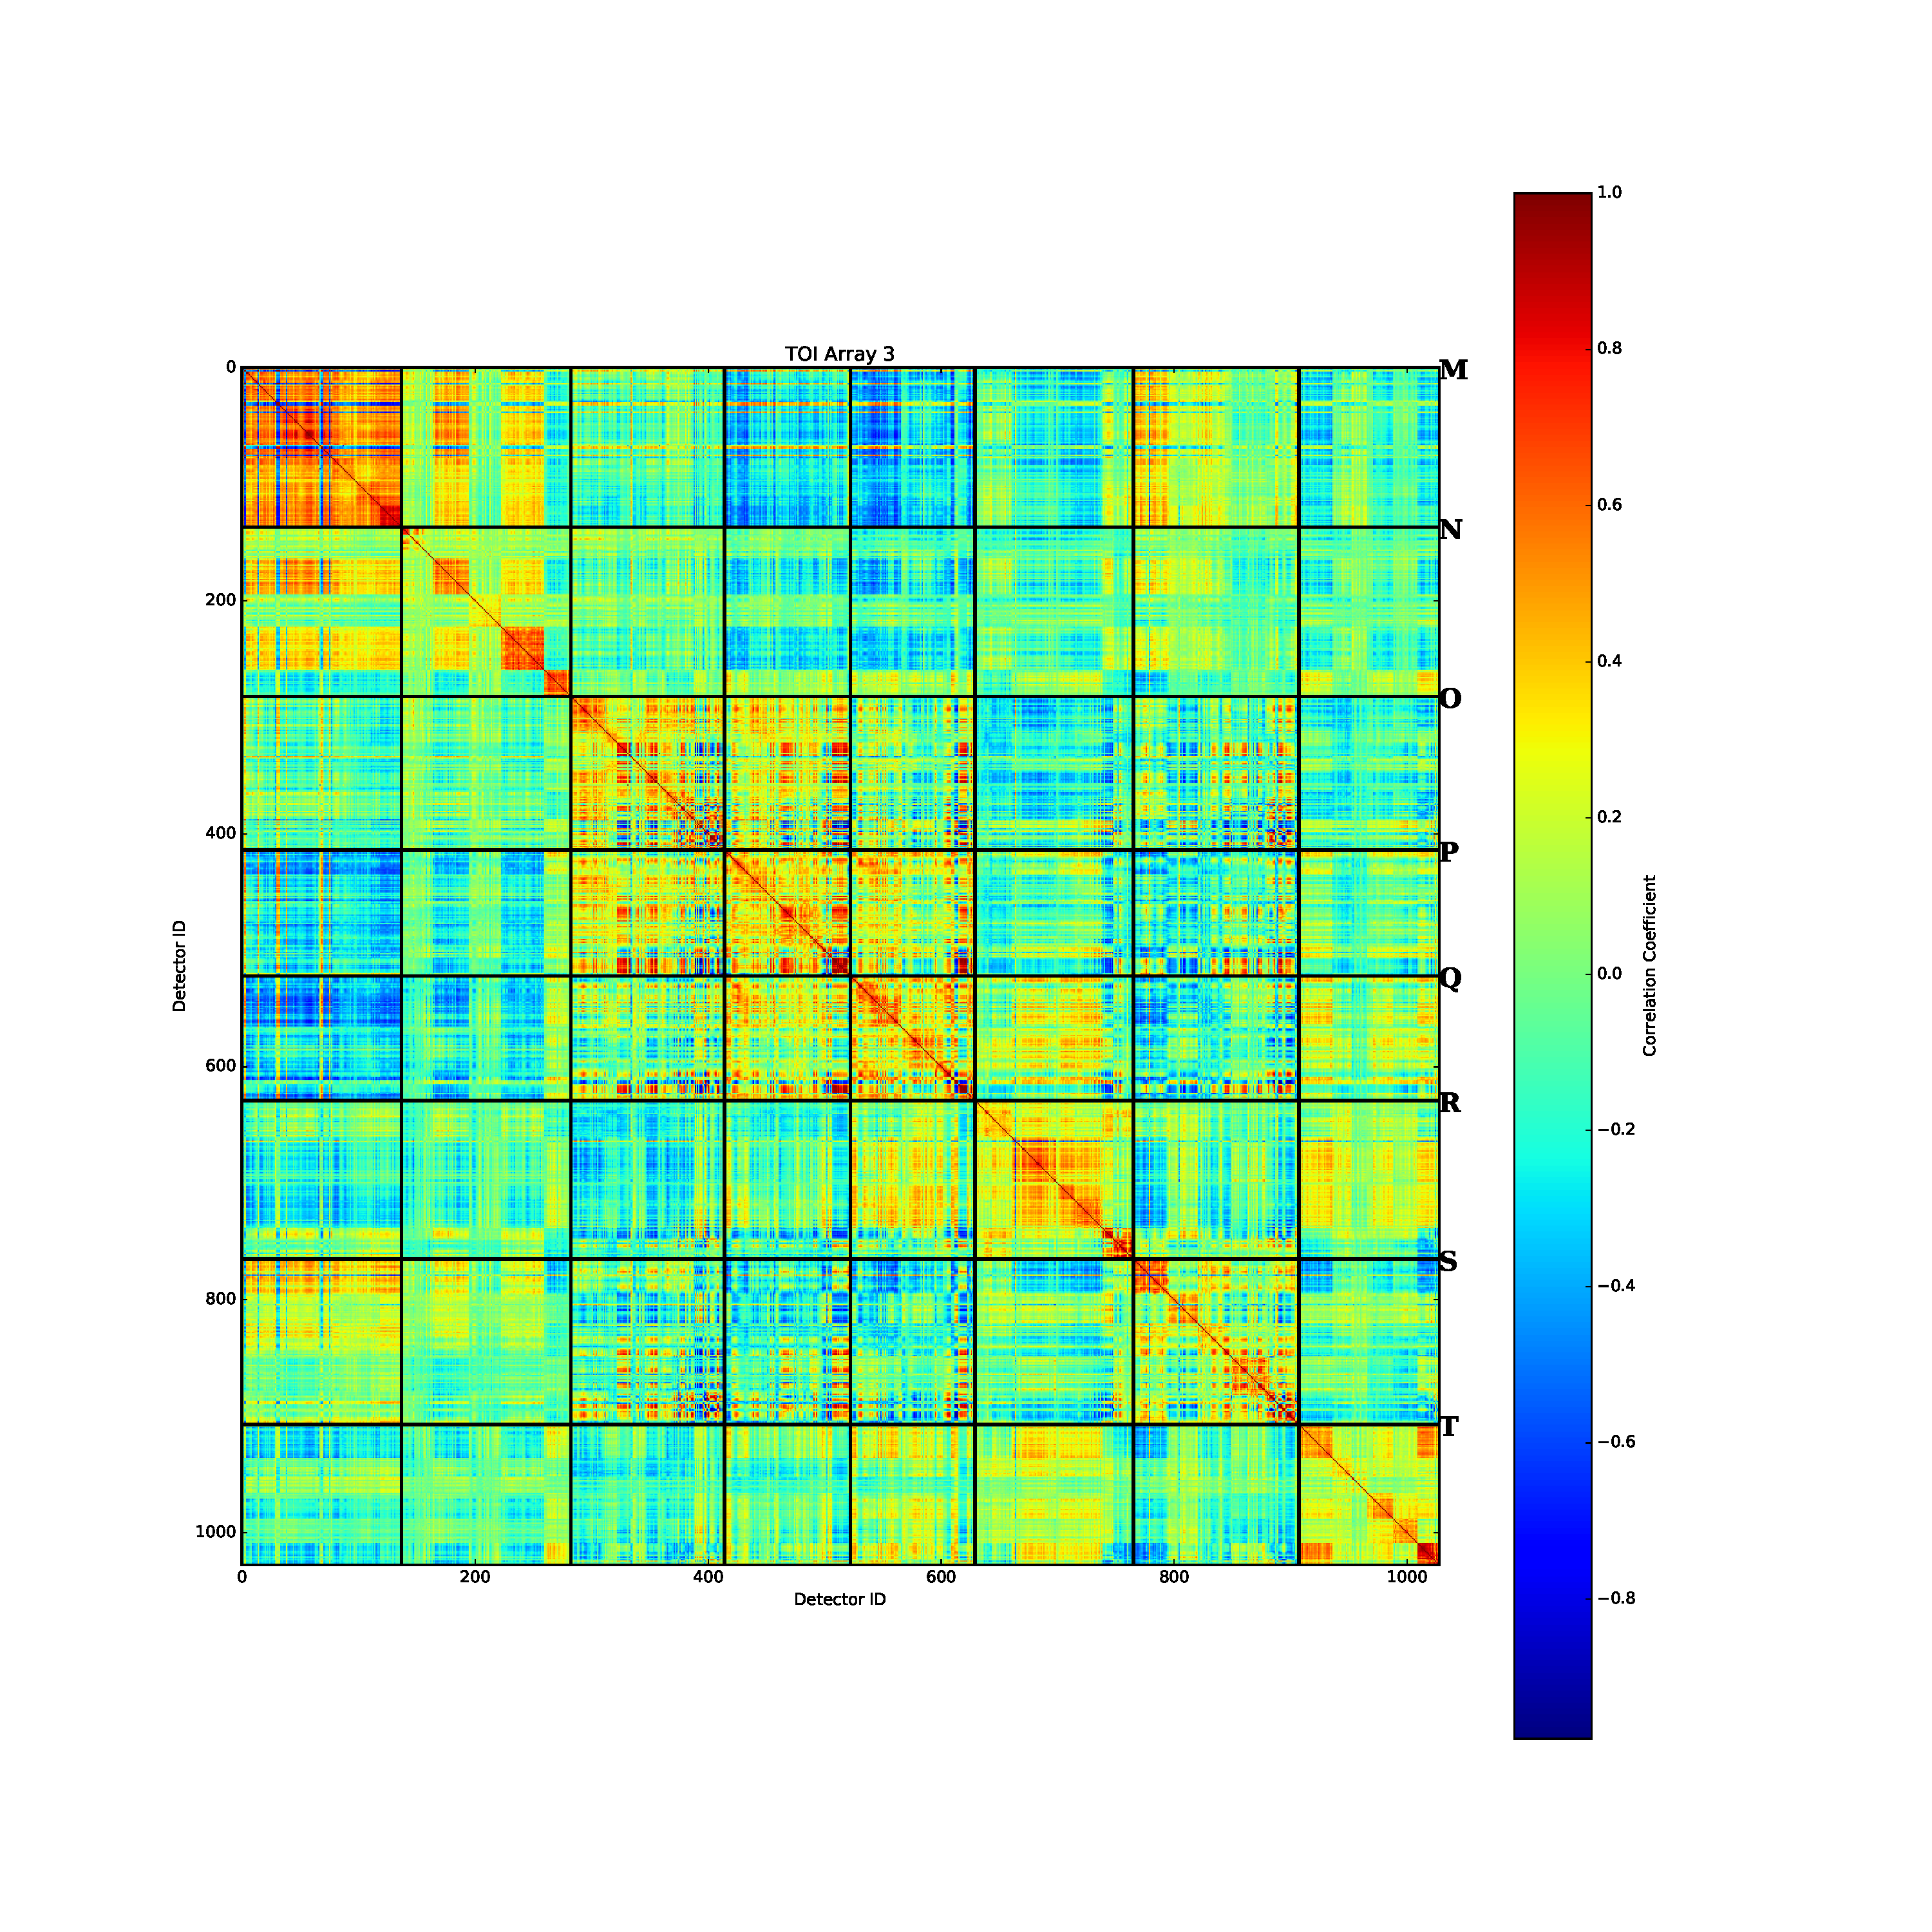
\includegraphics[width=0.3\textwidth]{Figures/DarkTests/corrmat_TOI_CM_array_3_20161213s72.pdf}
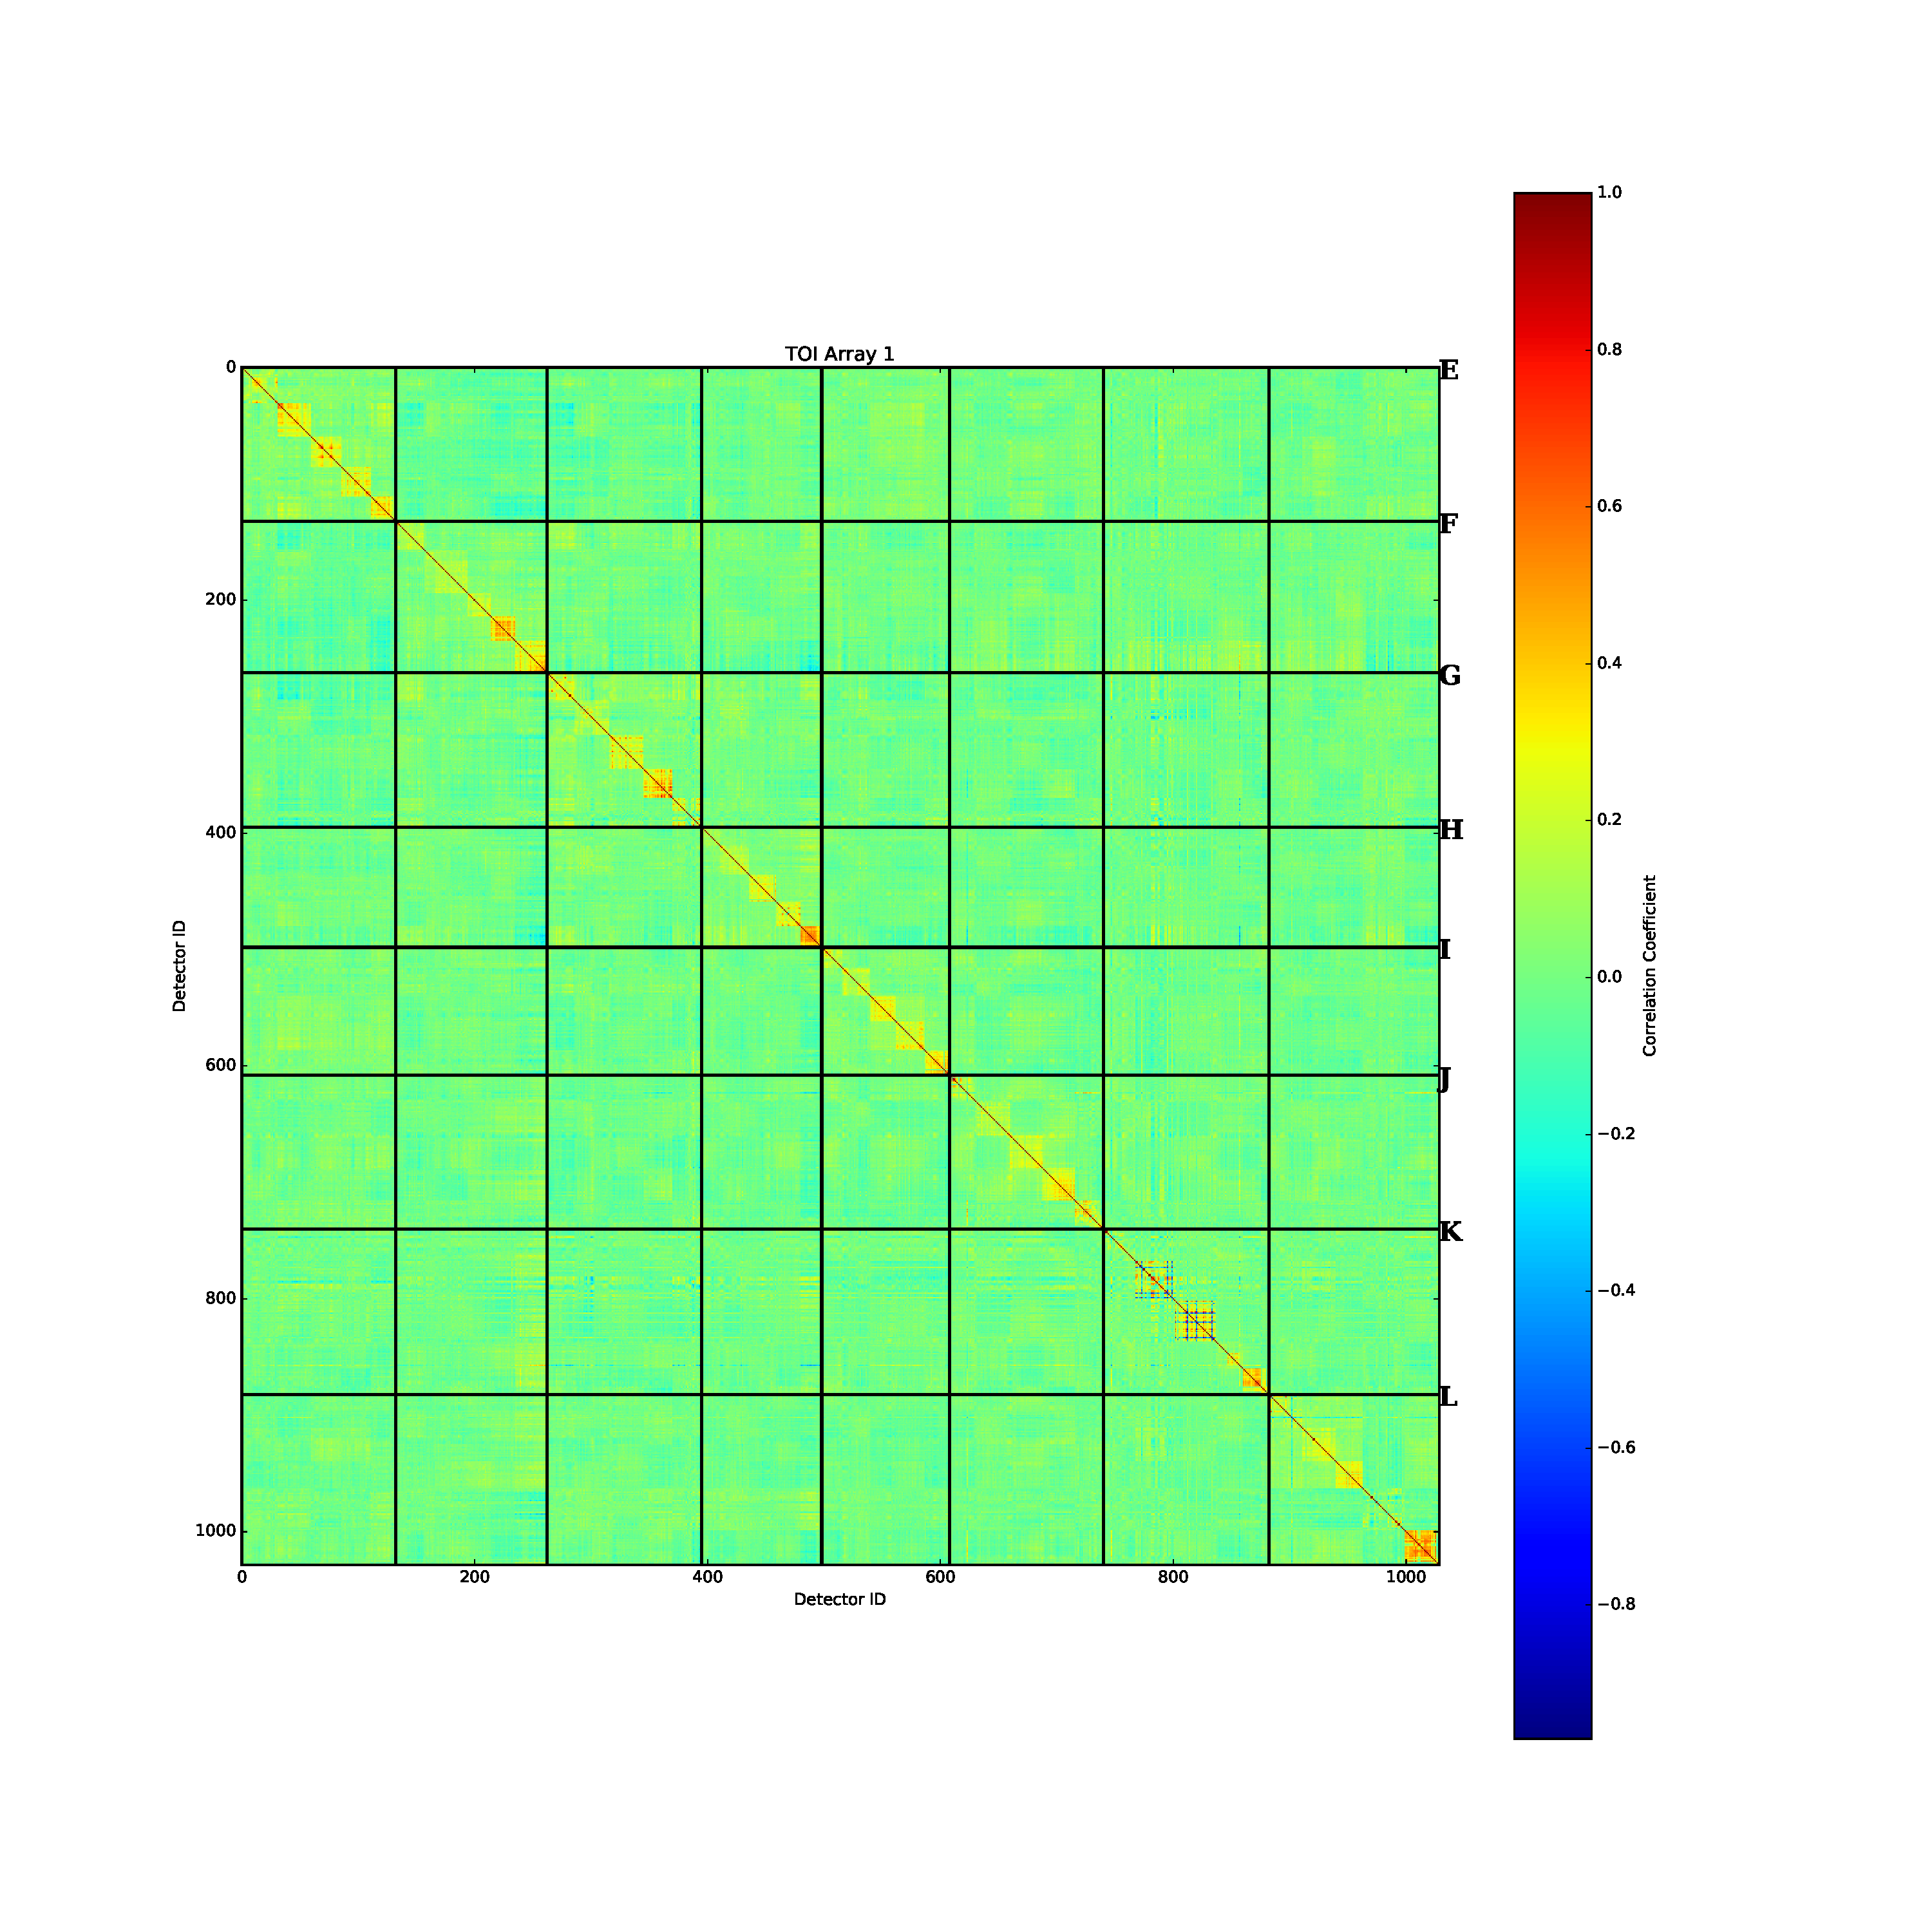
\includegraphics[width=0.3\textwidth]{Figures/DarkTests/corrmat_TOI_PCA_array_1_20161213s72.pdf}
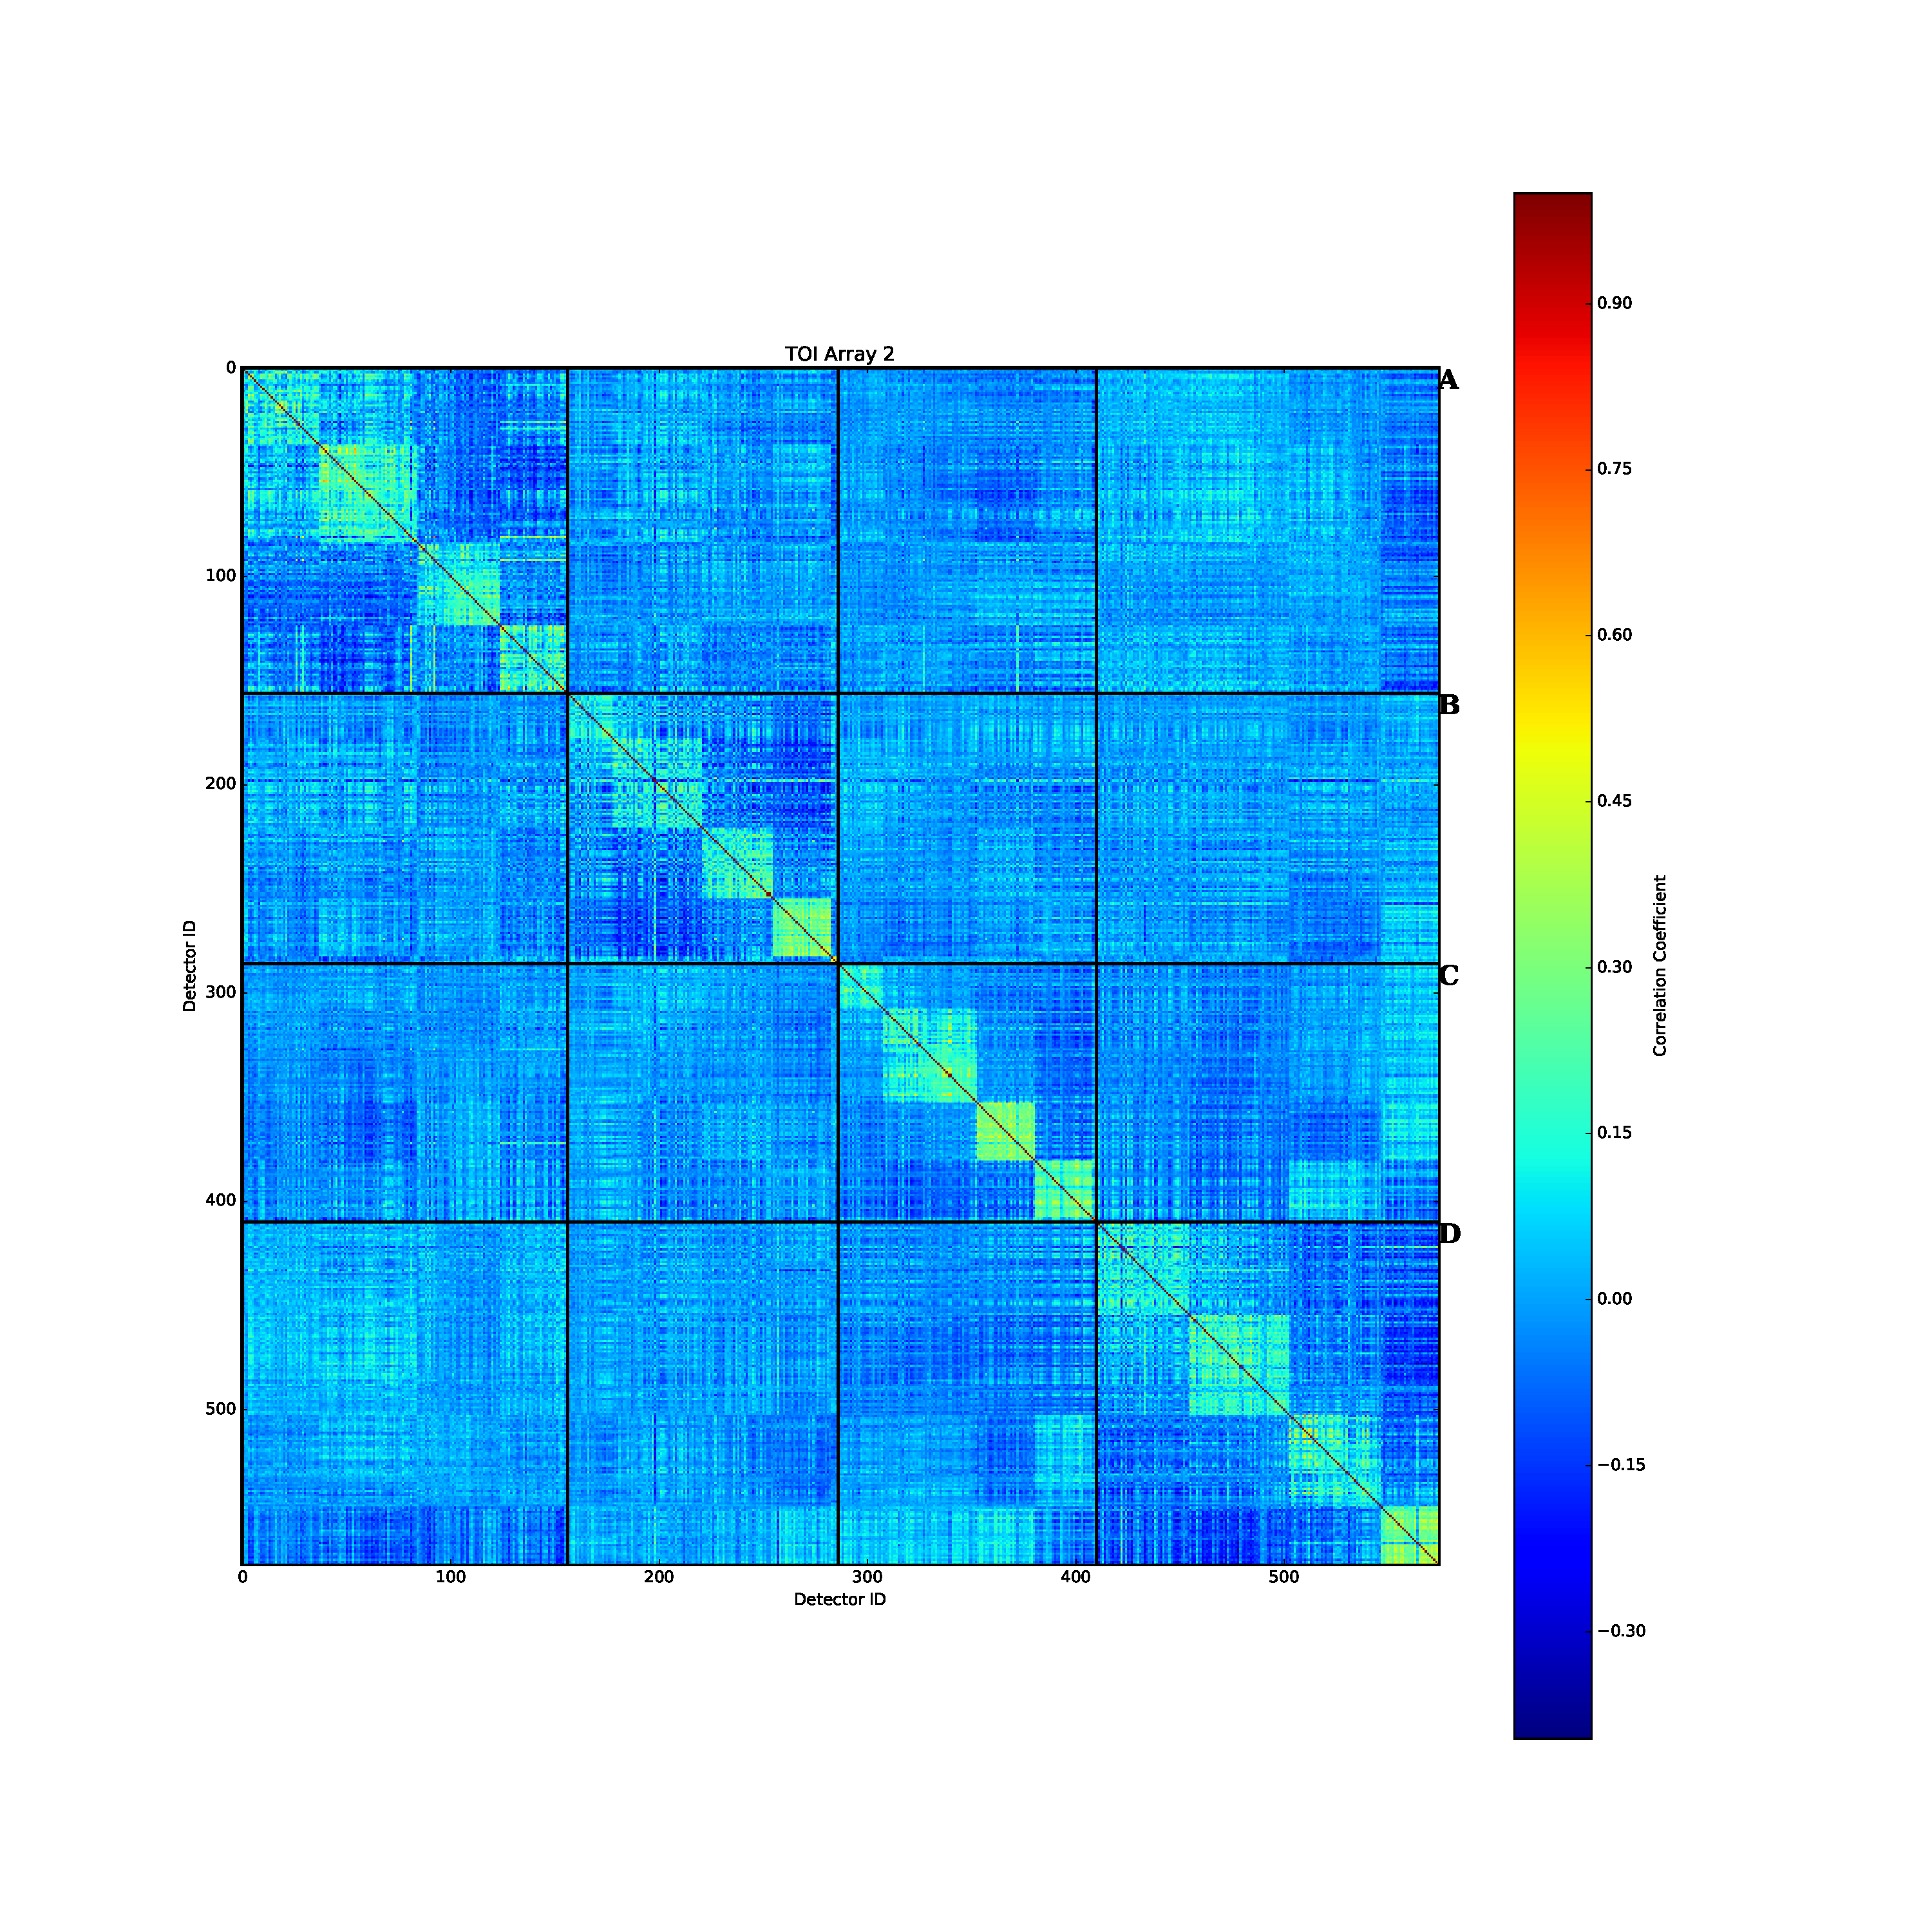
\includegraphics[width=0.3\textwidth]{Figures/DarkTests/corrmat_TOI_PCA_array_2_20161213s72.pdf}
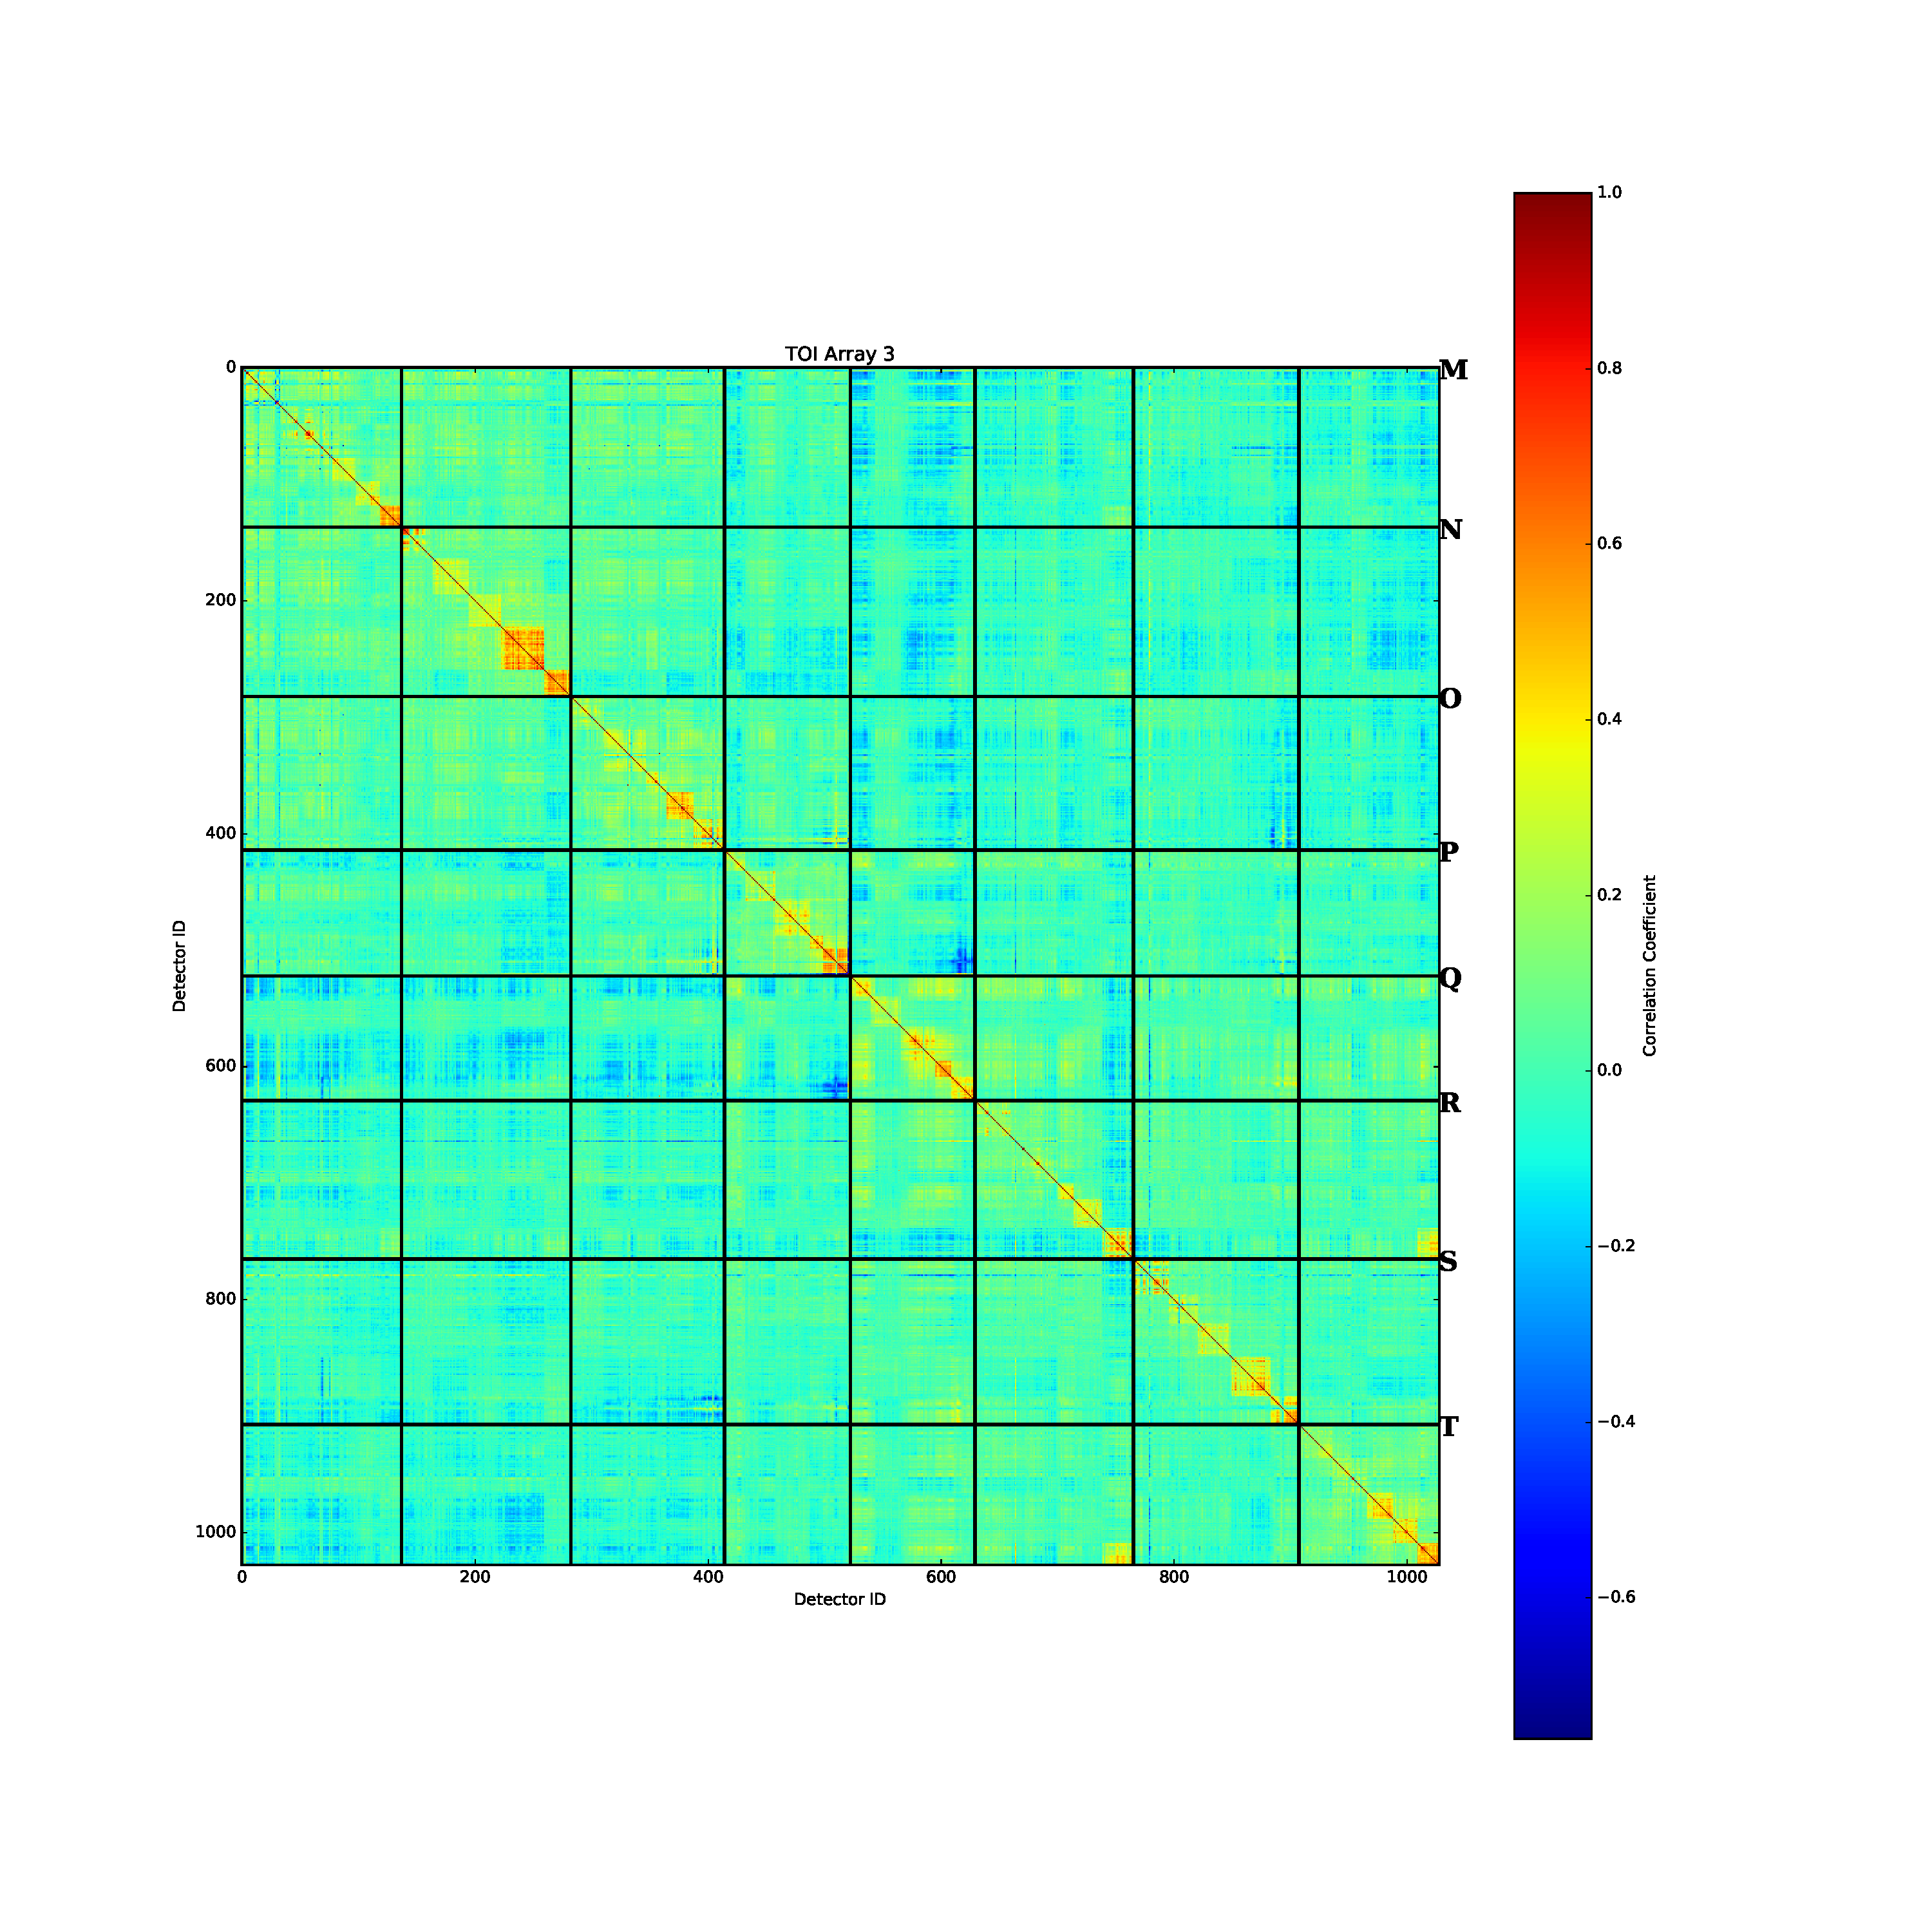
\includegraphics[width=0.3\textwidth]{Figures/DarkTests/corrmat_TOI_PCA_array_3_20161213s72.pdf}
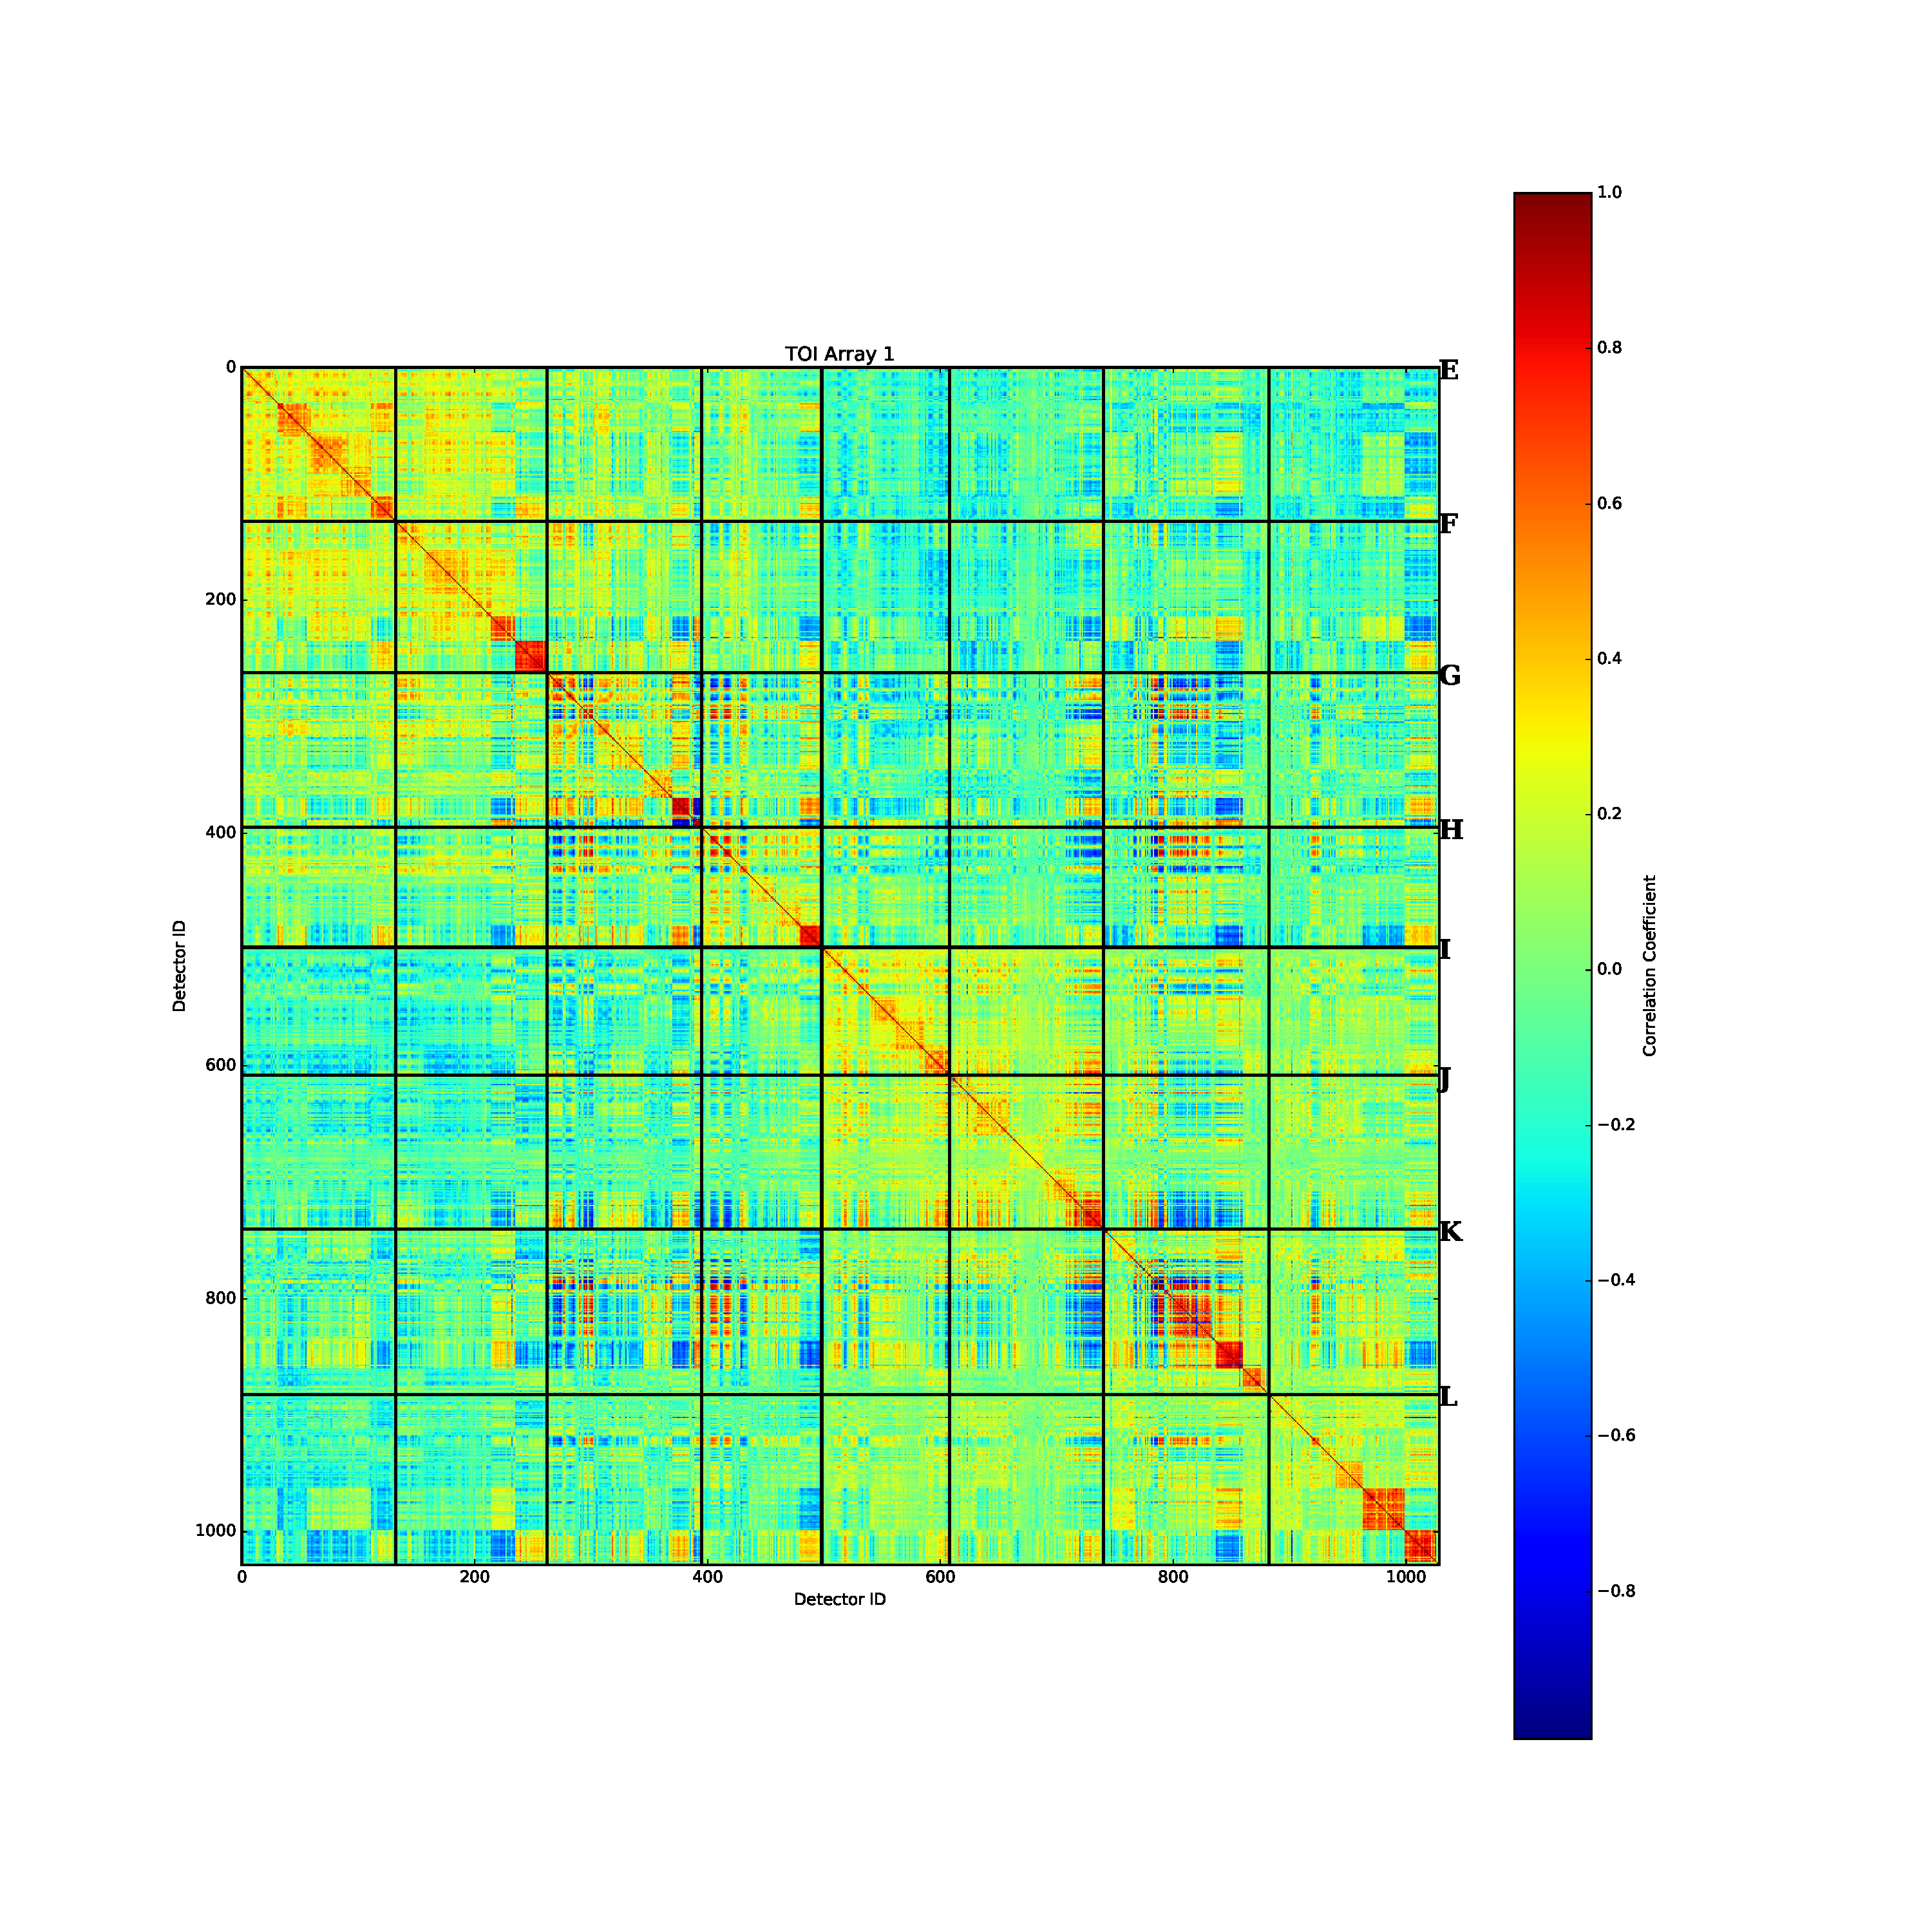
\includegraphics[width=0.3\textwidth]{Figures/DarkTests/corrmat_TOI_BC_array_1_20161213s72.pdf}
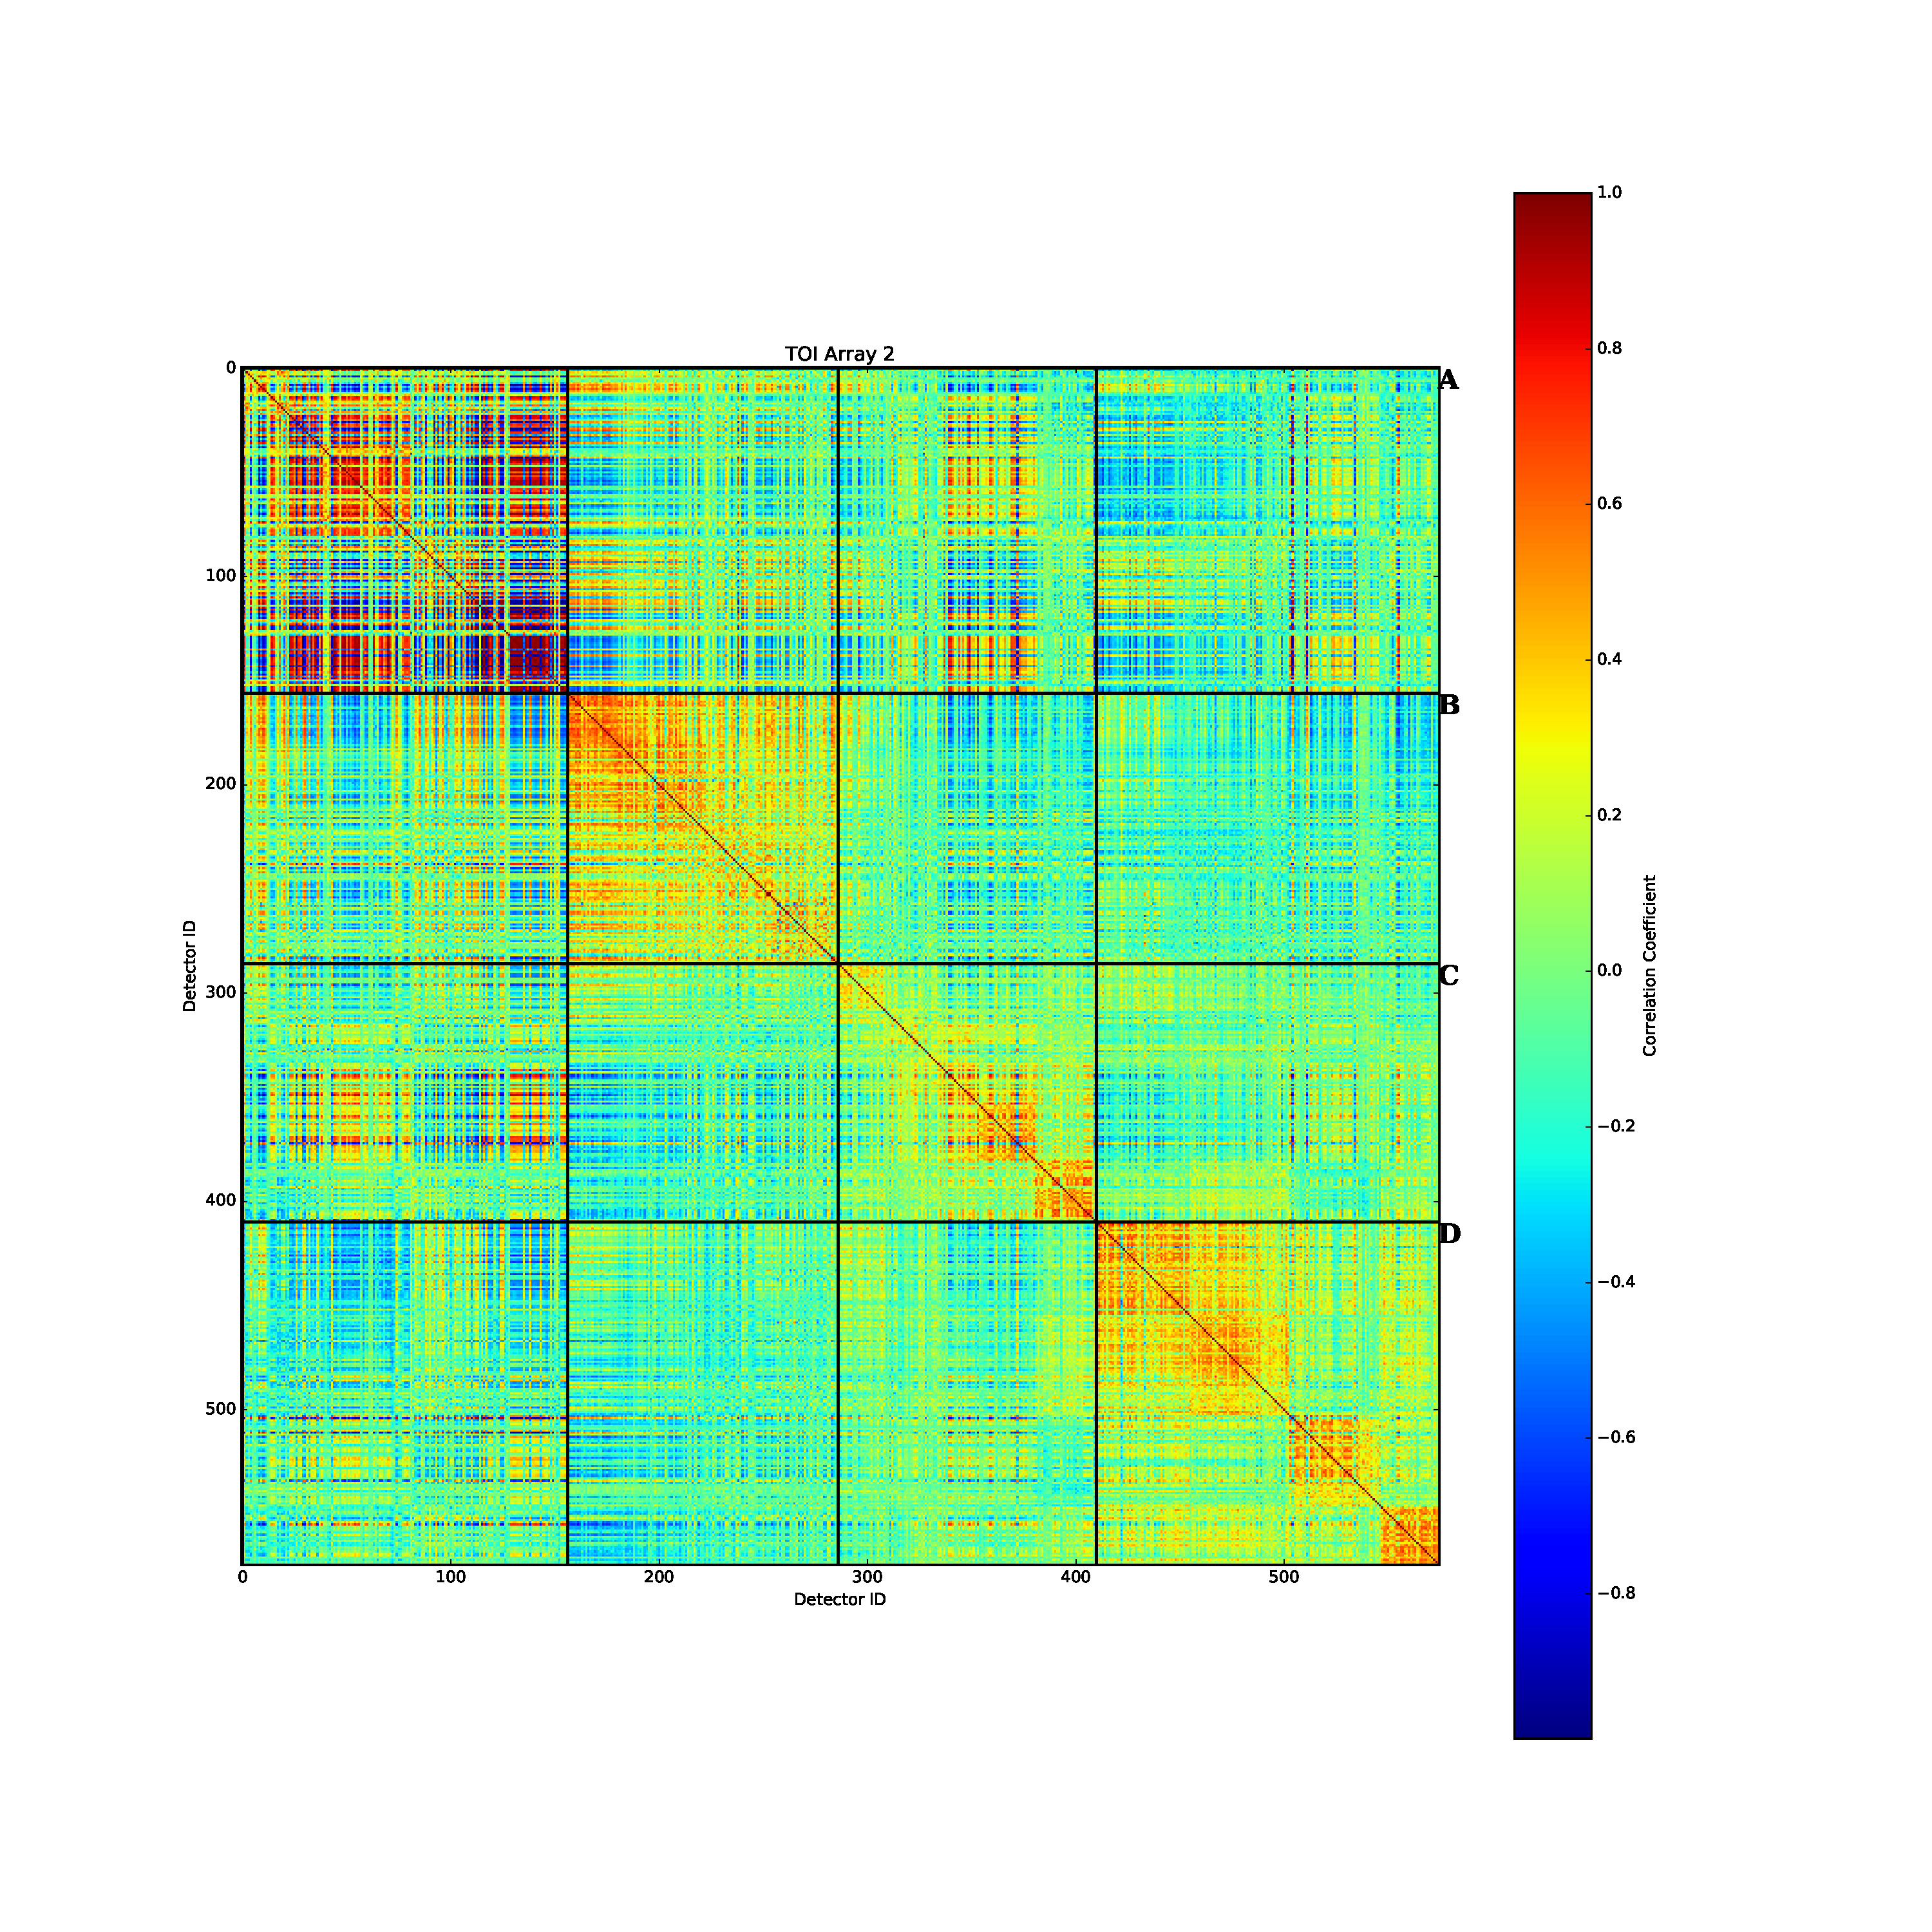
\includegraphics[width=0.3\textwidth]{Figures/DarkTests/corrmat_TOI_BC_array_2_20161213s72.pdf}
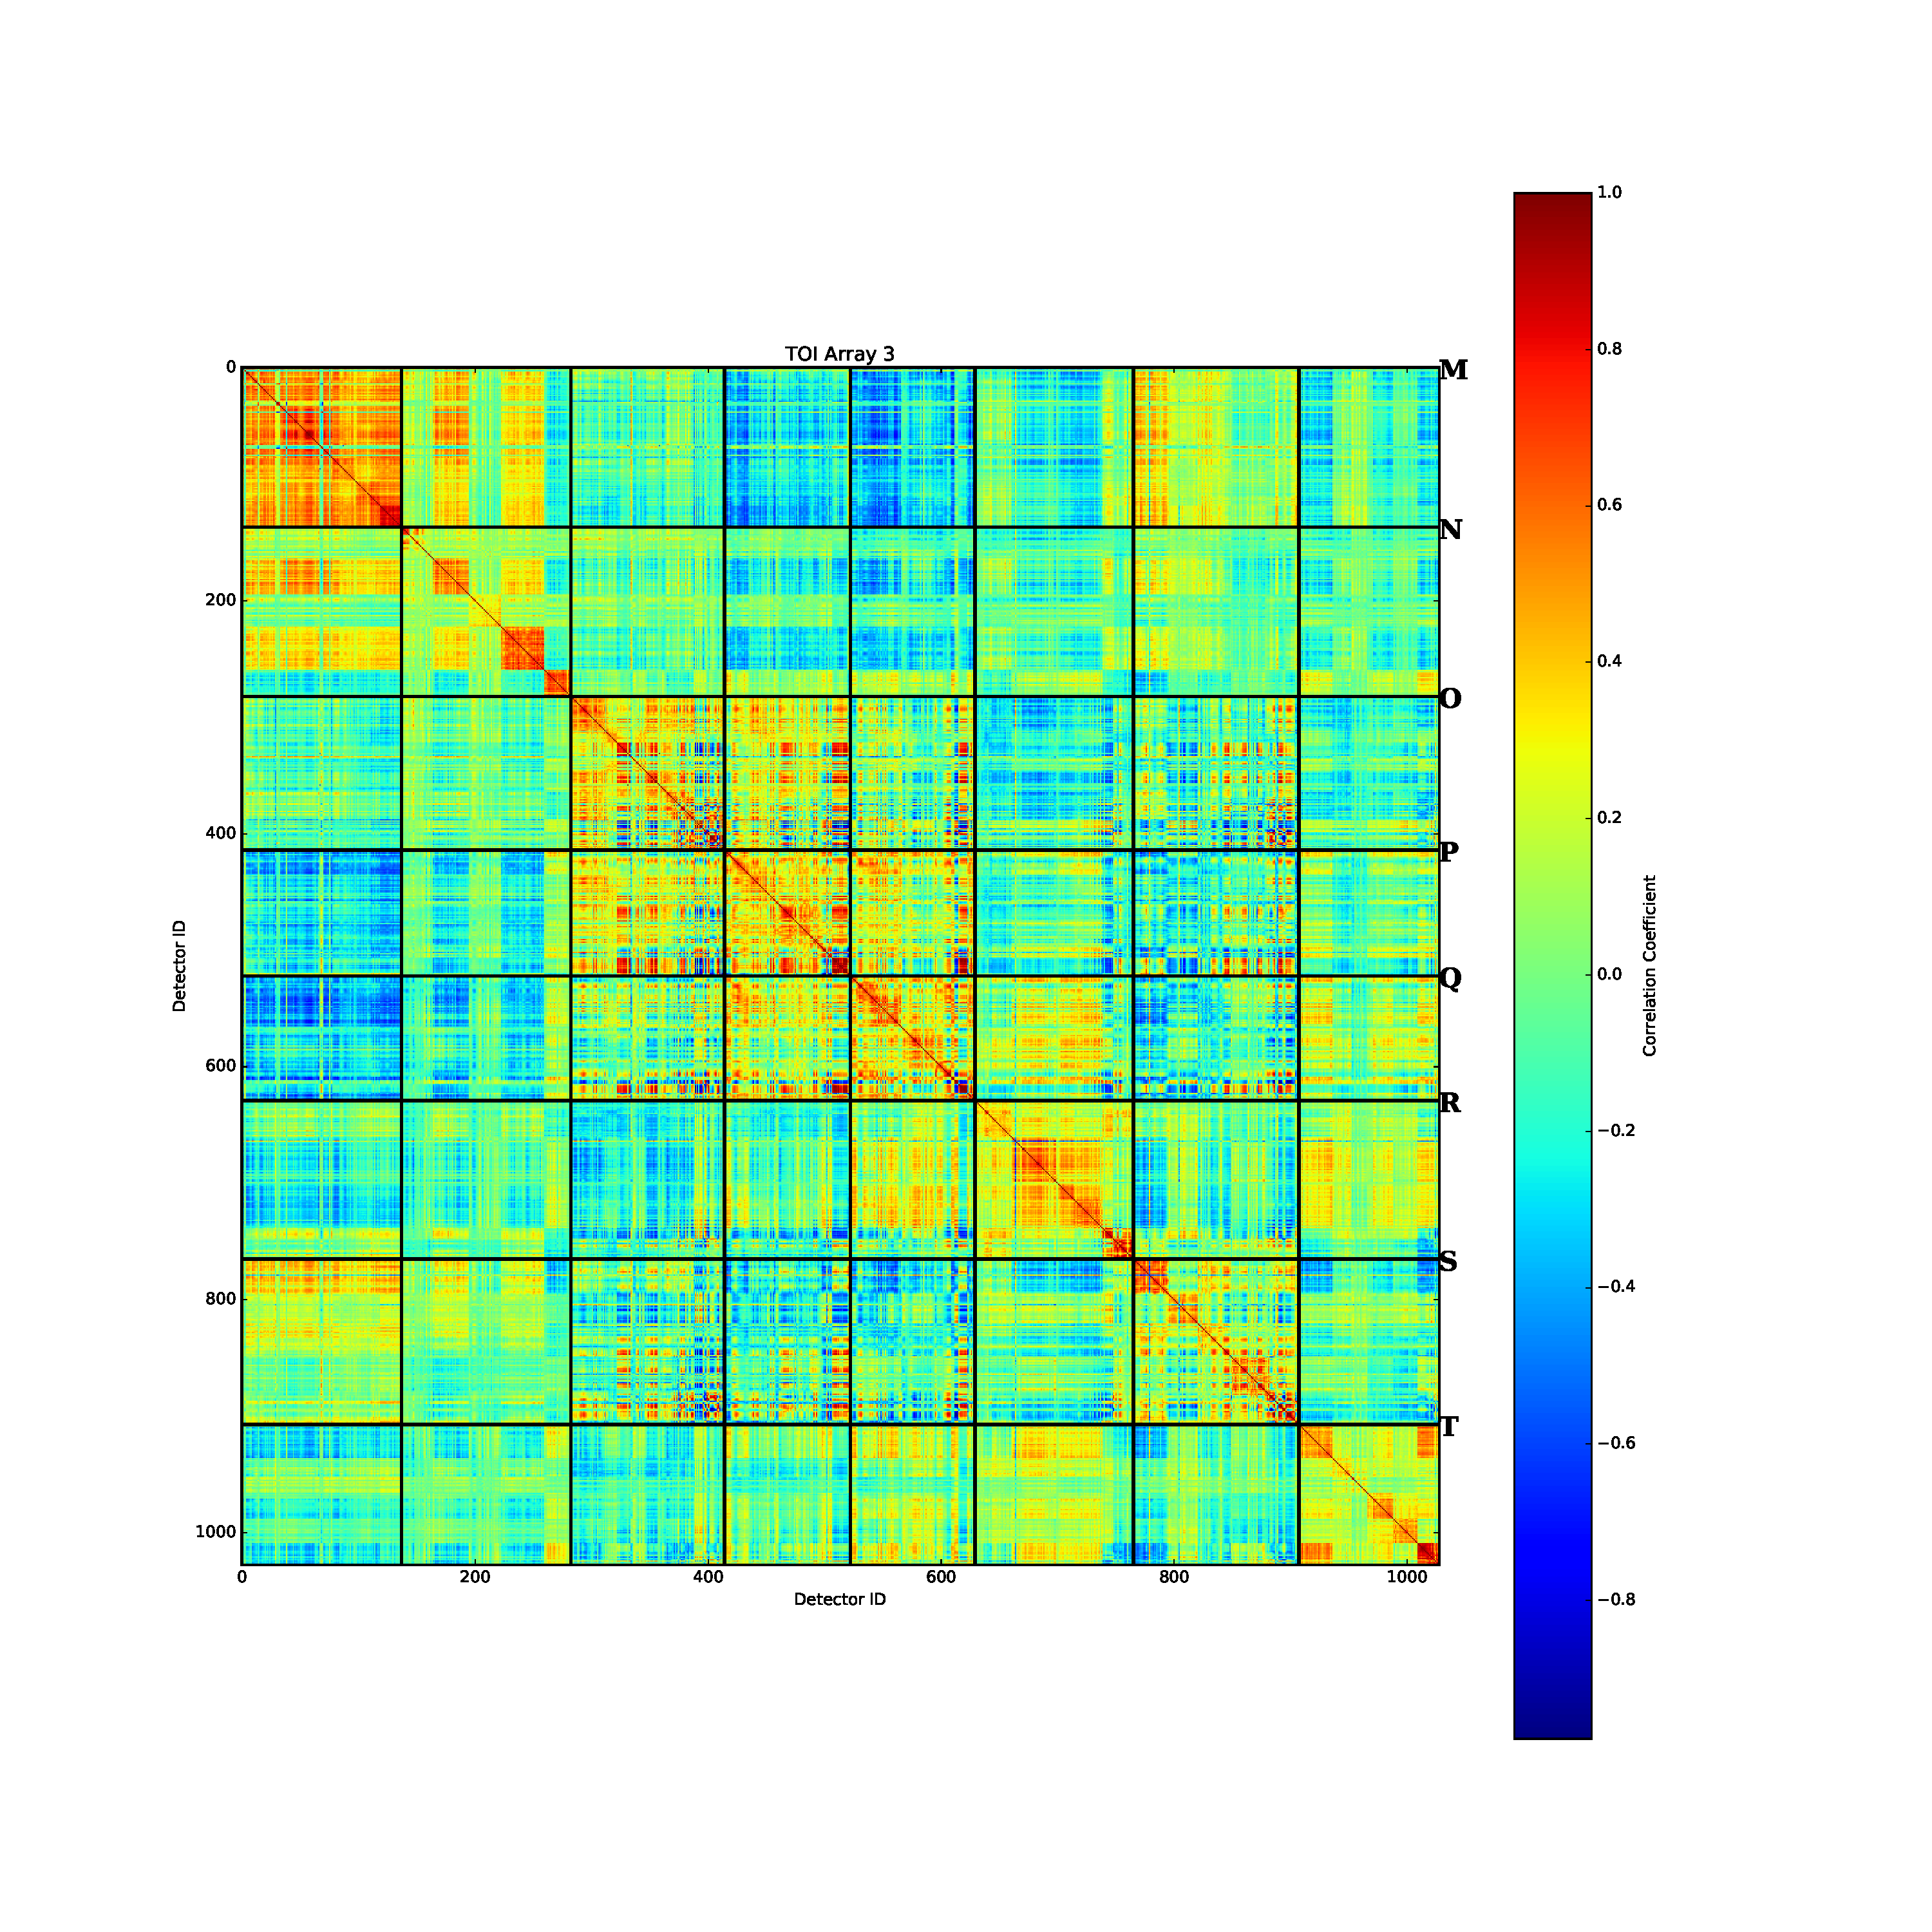
\includegraphics[width=0.3\textwidth]{Figures/DarkTests/corrmat_TOI_BC_array_3_20161213s72.pdf}
\end{center}
\caption{From left to right correlation matrices for the three NIKA2 arrays (A1, A2, and A3) for scan 20161213s72. From top to bottom we present the correlation of the raw data, after CM, PCA and BC decorrelations. \label{corrs72}}
\end{figure}

Using faint source measurements we have identified several noise components that require using complex decorrelation methods. Event in the case of multiple template decorrelation we find residual correlation between detectors that seems to be related to electronic subbands. We find significant differences between N2R4 and N2R7 scans. \\

After decorralation using multiple template procedures we reduce significantly the rms of the noise. In the case of dark test it becomes of the level of the high frequency noise. For faint source scans we also diminish the high frequency noise, which is probably dominated by atmospheric emission. We find significant differences between the noise levels in A1 and A3, which might be explained by gain differences (to be verified). For some electronic boxes in A2 the rms noise is significantly larger than for the others. For the three arrays we find increasing noise with increasing resonant frequency withing each electronic box.This is probably related to the difference of gains between subbands in the electronics. Furthermore, we find in A1 and A3 extra low frequency structures in the rms which are not identified yet.


